% =====================================================================
% Paper B — Systems (MDPI), SI "Using Digital AI Systems as a Response
% to High Economic Turbulence and Uncertainty"
%
% Audit framing (2026-10-05). Supersedes paper-v1-fragility.tex.
% Evidence: ../explore/rq1-floor-results.md; outline: ../plan/audit-outline.md.
% =====================================================================

\documentclass[systems,article,submit,moreauthors,pdftex]{Definitions/mdpi}

% --- Compatibility guards (no-ops under the current MDPI class) ---
\providecommand{\TitleCitation}[1]{}
\providecommand{\AuthorCitation}[1]{}
\providecommand{\orcidA}{}
\providecommand{\orcidB}{}
\providecommand{\orcidC}{}
\providecommand{\dataavailability}[1]{\vspace{6pt}\noindent\textbf{Data Availability Statement:} #1\par}
\providecommand{\institutionalreview}[1]{\vspace{6pt}\noindent\textbf{Institutional Review Board Statement:} #1\par}
\providecommand{\informedconsent}[1]{\vspace{6pt}\noindent\textbf{Informed Consent Statement:} #1\par}

\usepackage{booktabs}
\usepackage{tabularx}
\usepackage{multirow}
\usepackage{amsmath}
\usepackage{amssymb}
\usepackage{xurl}
\usepackage{tikz}
\usetikzlibrary{positioning,arrows.meta}

\graphicspath{{../figures/audit/}{../figures/}}

\Title{Is the Optimiser Needed? Auditing a Digital Decision-Support System for Necessity, Decision Stability and Input Fragility under Turbulence}
\TitleCitation{Is the Optimiser Needed? Auditing a Digital Decision-Support System under Turbulence}

\newcommand{\orcidauthorA}{0000-0002-1551-419X}% Vladimir Stantchev
\newcommand{\orcidauthorB}{0000-0003-1534-6680}% Peyman Rabiei
\newcommand{\orcidauthorC}{0000-0003-0292-7435}% Daniel Arias-Aranda

\Author{Vladimir Stantchev $^{1,}$*\orcidA{}, Peyman Rabiei $^{2}$\orcidB{} and Daniel Arias-Aranda $^{2}$\orcidC{}}
\AuthorNames{Vladimir Stantchev, Peyman Rabiei and Daniel Arias-Aranda}
\AuthorCitation{Stantchev, V.; Rabiei, P.; Arias-Aranda, D.}

\address{%
$^{1}$ \quad Institute of Information Systems, SRH University Heidelberg, Heidelberg, Germany; stantchev@computer.org\\
$^{2}$ \quad Faculty of Economics and Business, University of Granada, Granada, Spain; prabiei@correo.ugr.es (P.R.); darias@ugr.es (D.A.-A.)}

\corres{Correspondence: stantchev@computer.org}

\abstract{%
Optimisation-based decision-support systems are adopted under turbulence on two untested
assumptions: that the problem needs their stochastic optimiser, and that their committed decision
is stable. We audit both, and input fragility, with a five-step protocol on our own published fuzzy
multi-objective relief-allocation system, using synthetic instances. Its model is separable: a
deterministic rule computes the exact optimum, which dominates 97--100\% of the published front
points; the same check shows that its prioritisation objective, as written, rewards directing the
people of lowest priority. Runs with different seeds commit to allocations differing for 83--94\% of
the people directed. The solver stops where the model is flat: allocations within 1\% of the
optimum already differ for a quarter to a third of the people, and an exact decider with a stated
tie-breaking rule commits to one allocation. On that decider,
regret from degraded data grows with turbulence and concentrates in a few inputs. A load-aware
repair stays exactly solvable at the target sizes; beyond them, a capacity-aware local search beats
the exact method under a one-minute limit, and the evolutionary system at every size. On two
further models, one a third-party benchmark, the protocol reaches different verdicts. Economic
turbulence is engaged by analogy of mechanism only.}

\keyword{digital AI systems; economic turbulence; uncertainty; systems methodology; algorithmic auditing; decision-support systems; multi-objective optimization; exact optimization; decision stability; solution multiplicity; data quality; humanitarian logistics}

% Highlights (required by the updated Systems template)
\addhighlights{yes}
\renewcommand{\addhighlights}{%

\noindent\textbf{What are the main findings?}
\begin{itemize}[labelsep=2.5mm,topsep=-3pt]
\item The audited relief-allocation model is separable: a deterministic rule computes its exact optimum, which dominates 97--100\% of the published evolutionary front points, and the same check shows that its prioritisation objective, as written, rewards directing the people of lowest priority.
\item Allocations from different seeds differ for 83--94\% of the people directed because the model is flat near its optimum; an exact decider with a stated tie-breaking rule commits to one allocation.
\end{itemize}\vspace{3pt}
\textbf{What are the implications of the main findings?}
\begin{itemize}[labelsep=2.5mm,topsep=-3pt]
\item Before an optimisation-based decision-support system is adopted, its structure, an exact or bounded reference, the multiplicity of near-optimal decisions and its selection rule should be checked; a stochastic optimiser is needed only where these checks leave a gap.
\item Under input errors, the loss of a noise-free exact decider grows with the error level in every condition tested and is close to additive across fields, which gives a per-input measure of how much data quality matters.
\end{itemize}
}

\begin{document}

% =====================================================================
\section{Introduction}\label{sec:intro}

Turbulence breaks two things at once: the balance between demand and capacity, and the
data a decision rests on. An uncertainty shock depresses activity because firms cannot
read their own situation~\cite{bloom2009uncertainty}, and that uncertainty can be measured
and tracked~\cite{baker2016epu}; supply networks that must stay viable through such
periods are asked to decide while their inputs are late, noisy or missing~\cite{ivanov2020viability,ivanov2020covid}.
Digital AI systems are increasingly placed in exactly this position. They ingest
situational data, search a large decision space, and commit to an allocation that people
then carry out~\cite{modgil2022ai,belhadi2024ai,pan2025aiusage}.

Adopting such a system rests on two assumptions that are rarely tested. The first is
\emph{necessity}: that the decision problem is hard enough to need the system's stochastic
optimiser, here a multi-objective evolutionary search, rather than an exact method. The
question concerns the optimiser, not the decision support around it: the fuzzy scoring that
turns situational data into objectives can be worth keeping even when the search is not. The
second assumption is \emph{decision stability}: that running the system again on the same
data commits to the same allocation. Reproducibility, which a fixed random seed guarantees,
is weaker. A seeded system repeats one run exactly, and the next seed, equally valid, may
commit to a different allocation. Where allocations differ, three causes have to be told
apart: the solver stopped far from the optimum, the model admits many allocations of almost
equal quality, or the rule that selects among them is unstated. If either assumption fails, a
system can pass every accuracy check and still be the wrong tool for a turbulent environment:
its quality is bought at a cost it did not need to pay, and its output is hard to justify to
the people it allocates.

This paper audits one such system, and the system is our own. The fuzzy multi-objective
allocation tool that directs affected people to relief centres after a disaster grew out of
our earlier models~\cite{rabiei2021vehicle,rabiei2023volunteer} and was published, with an
open-source reference implementation, as a reproducible four-objective
framework~\cite{rabiei2026resilient}. It combines Mamdani fuzzy inference with NSGA-II and
NRGA, runs on a laptop, and its runs are bit-for-bit reproducible. The tool has been released
and tested on synthetic instances; we know of no operational use, and we do not claim one. We
expected an audit of its behaviour under input turbulence to confirm that the fuzzy front-end
makes the system degrade gracefully. It did not, and the reason was not where we looked first.

We report the audit as a reusable protocol of five steps: a structural check of the
optimisation model, an exact reference and dominance test, a decision-stability test of the
committed output, an input-turbulence study on a noise-free decider, and a repair with a
deployment envelope. Relief allocation after a disaster is an acute resource-allocation shock,
and it is the case of this paper. We relate it to economic turbulence only by mechanism
(Section~\ref{sec:case}): no market data enter the audit, and no number in it is a claim about
markets or about commercial systems. To show that the protocol does more than detect one
defect, we also run it on two further models whose structure differs: the ED volunteer-staffing
model from which the relief tool grew~\cite{rabiei2023volunteer}, where the choices are coupled
by a one-to-one matching, and a multi-objective knapsack benchmark that is not ours and whose
weighted sums are NP-hard~\cite{zitzler1999spea}.

Four research questions structure the audit:
\begin{itemize}
\item[RQ1] (\emph{Necessity}) Does the published optimisation model require the evolutionary
search?
\item[RQ2] (\emph{Decision stability}) Does the system commit to the same allocation when run
again on the same data, and if not, how much of the difference is due to the solver and how
much to the model?
\item[RQ3] (\emph{Input fragility}) How much does a decision lose when it is made on degraded
data, once solver noise is removed?
\item[RQ4] (\emph{Repair and envelope}) Does a minimal semantic repair of the model change
these answers, and where does exact optimisation stop being practical?
\end{itemize}

The answers are uncomfortable for the system and useful for its users. The published model
is separable: a deterministic greedy rule computes the exact optimum of any weighted
objective sum in milliseconds, and one such point dominates 97--100\% of the front points the
evolutionary solvers returned in our own published experiments. The committed decision of the
evolutionary system differs for most of the directed people between two runs on identical
data, and the model itself admits allocations within one objective unit of the optimum that
differ for a quarter to a third of them; an exact decider with a stated tie-breaking rule
commits to one allocation. Measured on the exact decider, the regret of deciding on degraded
data grows smoothly and is concentrated in the inputs the objectives consume. A minimal repair
that makes one objective depend on the load it creates restores the intended direction, and
the repaired model is still solved exactly at the sizes the system targets; beyond them a
capacity-aware local search beats the exact method under a one-minute limit and the audited
evolutionary system at every size. The structural check also shows that, as written, the published
prioritisation objective rewards directing the people of lowest priority.

What is new is not the correction of our earlier study, which follows from the first step, but
four things that the correction does not supply: a protocol whose steps each end in a
checkable number and that branches differently on models of different structure; a
decomposition of decision instability into solver variance, model multiplicity and selection
policy, with a tie-breaking rule that removes the last; a measure of input fragility on a
noise-free decider, which separates it from the solver's own variance; and a deployment
envelope that compares exact and heuristic methods at equal end-to-end latency. The open
artefact makes each finding checkable.

The work belongs to systems practice: it audits a decision system as a whole, from data
through fuzzy scores, objective model, search and selection rule to the committed allocation,
and it is meant for the point where an organisation decides whether to adopt such a system
for a turbulent environment. Section~\ref{sec:background} positions the audit;
Section~\ref{sec:case} describes the system, its model and the turbulence mapping;
Section~\ref{sec:protocol} defines the protocol; Section~\ref{sec:results} reports RQ1--RQ4
and the two further cases; Sections~\ref{sec:discussion} and~\ref{sec:conclusion} draw the
implications.

% =====================================================================
\section{Background}\label{sec:background}

\subsection{Decision systems under deep uncertainty}
A decision aid can absorb only as much environmental variety as it can represent; Ashby's
law of requisite variety~\cite{ashby1956cybernetics} is the systems statement of that
limit, and bounded rationality~\cite{simon1955behavioral} is its behavioural counterpart.
Operational research answered with robustness as a criterion in its own
right~\cite{rosenhead1972robustness}, with warnings against models that are elegant but
detached from the problem they claim to represent~\cite{ackoff1979future}, and, more
recently, with methods that evaluate decisions across many plausible futures rather than
one forecast~\cite{lempert2006robust,walker2003uncertainty,marchau2019deep}. Robust
optimisation turns the same concern into tractable models~\cite{bental2002robust,bertsimas2004price}.
Our audit borrows the stance and applies it to the decision system itself: before asking
how a system responds to turbulence, ask whether its structure matches the problem.

\subsection{Multi-objective search, exact methods and their critique}
Multi-objective evolutionary algorithms such as NSGA-II~\cite{deb2002nsga2}, NRGA~\cite{aljadaan2008nrga}
and NSGA-III~\cite{deb2014nsga3} return an approximation of the Pareto front and leave the
final commitment to a selection rule~\cite{branke2004knees}. Their behaviour under noisy
fitness and uncertain parameters is well studied~\cite{jin2005uncertain,deb2006robustness,beyer2007robust,ide2016robustness},
and front quality is commonly measured by hypervolume~\cite{zitzler1999spea}. The theory of
multicriteria optimisation is equally clear that weighted-sum scalarisation recovers every
supported Pareto point~\cite{ehrgott2005multicriteria,das1998nbi}, and exact methods for
multi-objective combinatorial problems are mature~\cite{ehrgott2000moco}. A heuristic must
therefore justify itself against an exact baseline~\cite{hooker1995testing}; no algorithm
is better than another across all problems~\cite{wolpert1997nfl}, so the choice should
follow from problem features~\cite{kerschke2019selection}. The metaheuristics community has
criticised the habit of skipping this step~\cite{sorensen2015metaphor,aranha2022metaphor},
and benchmarking guidelines now require seeds, baselines and complete
reporting~\cite{bartzbeielstein2020benchmarking}. Reproducibility of evolutionary
computation, including the dependence of outcomes on random seeds, has its own
literature~\cite{lopezibanez2021reproducibility}.

\subsection{Fuzzy inference in decision support}
Fuzzy sets~\cite{zadeh1965fuzzy} and Mamdani inference~\cite{mamdani1975linguistic} encode
expert judgement as linguistic rules over graded memberships, and fuzzy multi-criteria
methods are widespread in decision support~\cite{kahraman2015fuzzymcdm}. Uncertainty in
the memberships themselves is the domain of type-2 systems~\cite{mendel2017uncertain,castillo2008type2}.
The audited system uses type-1 Mamdani inference, implemented with
scikit-fuzzy~\cite{warner2019skfuzzy}, to turn situational inputs into objective scores.

\subsection{Humanitarian operations}
Disaster operations research has a long review
tradition~\cite{altay2006ormsdisaster,galindo2013review,caunhye2012emergency}, and
post-disaster logistics differs structurally from commercial logistics through demand
surges, deprivation and degraded information~\cite{holguinveras2012unique,kovacs2007humanitarian,sheu2007emergency}.
Practitioners weigh several objectives at once~\cite{gralla2014tradeoffs}, multi-criteria
models are common~\cite{gutjahr2016multicriteria}, and the field has asked for models that
are implementable rather than only elegant~\cite{besiou2020humanitarian}. Closest to the
audited problem, volunteer and resource assignment under uncertainty has been solved
exactly by robust optimisation~\cite{lassiter2015volunteer}. Resilience
framings~\cite{bruneau2003resilience,christopher2004resilient,sheffi2005resilient,hosseini2019review}
connect these operations to the supply-chain literature on
disruption~\cite{queiroz2022epidemic,aghsami2024humanitarian}.

\subsection{Data quality, trust and auditing of AI systems}
Data quality has several dimensions, among them accuracy, completeness and
timeliness~\cite{wang1996dataquality}, and in high-stakes AI upstream data problems
compound into downstream harm~\cite{sambasivan2021cascades}. Deployment conditions differ
from development conditions~\cite{quinonerocandela2008shift,amodei2016concrete}.
Trust in an AI system is warranted only when the system has the properties the trust
assumes~\cite{jacovi2021trust}, and accountability requires decision procedures that can
be verified after the fact~\cite{kroll2017accountable,doshivelez2017interpretable}.
Algorithmic auditing turns these demands into procedures, from internal end-to-end
frameworks~\cite{raji2020audit} to ethics-based~\cite{mokander2021ethics} and external
audits~\cite{metaxa2021auditing}; production-readiness tests do the same for machine-learning
pipelines~\cite{breck2017mltestscore}. Regulation now codifies risk-management, data-governance,
record-keeping, accuracy and robustness duties for high-risk systems~\cite{eu2024aiact}, and
management-system and risk standards~\cite{iso2023aims,iso2023airisk,nist2023airmf} turn them
into organisational processes, while computational science treats reproducibility as a
precondition of trust~\cite{peng2011reproducible,stodden2016enhancing,gundersen2018reproducibility,pineau2021reproducibility,wilkinson2016fair}.
How wrong operational data are in practice has been measured only in a few settings. In
retail supply chains, about two thirds of store-level inventory records disagreed with the
physical stock~\cite{dehoratius2008inventory}; after the 2010 Haiti earthquake, gaps in
information and in its exchange between organisations hampered the humanitarian
response~\cite{altay2014haiti}. Neither gives error magnitudes per field of the kind a
perturbation study would need.

\subsection{Multiplicity of near-equivalent solutions}
Machine learning knows the problem of many good answers as the Rashomon
effect~\cite{breiman2001twocultures}: many models fit the data almost equally well. Predictive
multiplicity measures how far such models disagree on individual
predictions~\cite{marx2020multiplicity}, the set of near-optimal models has been
characterised~\cite{semenova2022rashomon,fisher2019allmodels}, and the consequences for
arbitrariness and accountability have been set out~\cite{black2022multiplicity}. Operational
research met the same question earlier from the other side: modelling to generate
alternatives searches deliberately for solutions that are near-optimal but maximally
different~\cite{brill1979public,brill1982mga}, and mixed-integer solvers can enumerate several
optimal or near-optimal solutions~\cite{danna2007multiple}. An allocation system inherits both
faces of the problem. Its model may admit many allocations of almost equal quality, and its
solver may land on any of them.

\subsection{Positioning}\label{sec:positioning}
Audits of AI systems mostly examine predictive models: their accuracy, fairness,
transparency and documentation. Optimisation-based decision systems raise two further
questions. Is the stochastic search needed at all, given the structure of the model? And is
the committed output stable, or one draw from a distribution of decisions?
Table~\ref{tab:positioning} maps the five steps of our protocol against the frameworks closest
to it. The structural check (S1) and the regret of a noise-free decider (S4) have no
counterpart. Benchmarking guidelines recommend exact baselines, but not a dominance test of the
committed system against them (S2). Frameworks that ask for robustness and consistency do not
separate solver variance from the multiplicity of the problem (S3).

\begin{table}[H]
\centering
\caption{The audit protocol against established frameworks. \checkmark: the framework asks
for this check; $\circ$: it asks for a related but weaker check; --: absent. EU AI Act
articles: 9 risk management, 10 data governance, 12 record-keeping, 15 accuracy and
robustness.\label{tab:positioning}}
\footnotesize
\begin{tabularx}{\textwidth}{>{\raggedright\arraybackslash}X *{5}{>{\centering\arraybackslash}p{1.75cm}}}
\toprule
Protocol step & SMACTR \cite{raji2020audit} & ML Test Score~\cite{breck2017mltestscore} & EU AI Act~\cite{eu2024aiact} & ISO/IEC 42001, 23894~\cite{iso2023aims,iso2023airisk} & Bench\-marking\newline\cite{hooker1995testing,bartzbeielstein2020benchmarking,beiranvand2017bestpractices}\\
\midrule
S1 Structure of the optimisation model & -- & -- & -- & -- & $\circ$\\
S2 Exact reference; dominance of the committed system & -- & -- & $\circ$ (Art.~15) & -- & $\circ$\\
S3 Stability of the committed decision; solver vs.\ problem multiplicity & -- & $\circ$ & $\circ$ (Art.~15) & -- & $\circ$\\
S4 Input degradation scored on a noise-free decider & $\circ$ & $\circ$ & $\circ$ (Art.~10, 15) & $\circ$ & --\\
S5 Repair; exact vs.\ search at equal latency & -- & $\circ$ & $\circ$ (Art.~9) & $\circ$ & $\circ$\\
Manifests, seeds, environment fingerprints & $\circ$ & \checkmark & \checkmark\ (Art.~12) & \checkmark & \checkmark\\
\bottomrule
\end{tabularx}
\end{table}

The protocol complements these frameworks rather than replacing them. It supplies the evidence
that an Article~15 robustness claim or an ISO/IEC 42001 risk treatment would need for a system
whose core is an optimiser rather than a predictor. Its new checkpoints are S1, the dominance
test of S2, the decomposition of S3 and the regret measure of S4.

% =====================================================================
\section{The Case: Relief Allocation as an Acute Turbulence Shock}\label{sec:case}

\subsection{The audited system}
The system directs $n_{\mathrm{dir}}$ of $m$ affected people to $n$ relief centres. It
reads per-person attributes (age, disability, injury and living status, local
infrastructure-damage level, remaining resource time), per-centre state (occupancy and
resource-depletion rates) and per-route data (travel duration, road condition, possible
hazard). Mamdani fuzzy inference systems turn these inputs into scores, and the scores
into objectives to be minimised: unfairness in prioritisation (ULPP), transport
infeasibility (TIL) and centre allocation imbalance (CAIL) in the three-objective
baseline, with TIL split into robustness and rapidity deficits in the four-objective
variant~\cite{rabiei2026resilient}. NSGA-II or NRGA search the allocations and return a
Pareto front (NSGA-III serves as a further control in this audit); a committal rule picks one allocation from it. The reference
implementation is open source, continuously tested and dependency-audited, and records a
SHA-256 signature of every front together with an environment fingerprint.

We audit the three-objective baseline at the two reference sizes of the published study:
\emph{small} (5 centres, 150 people, 50 directed) and \emph{large} (10 centres, 300
people, 100 directed). Where a finding concerns the published experiments, we also check
the four-objective variant and the medium size.

\subsection{The model}\label{sec:model}
This subsection states the audited model as the reference implementation computes it. The
membership functions and rule bases are those of~\cite{rabiei2026resilient}; the full rule
tables are given there.

\subsubsection{Decision and inputs}
Let $J=\{1,\dots,m\}$ index the affected people and $I=\{1,\dots,n\}$ the relief centres, with
$0<n_{\mathrm{dir}}<m$. A decision $d=(D,c)$ is a set $D\subset J$ of exactly $n_{\mathrm{dir}}$
directed people and an assignment $c\colon D\to I$ of each directed person to one centre;
equivalently $x_{j,i}\in\{0,1\}$ with $\sum_{i}x_{j,i}\le 1$ for every $j$ and
$\sum_{j,i}x_{j,i}=n_{\mathrm{dir}}$. People outside $D$ are not directed. The published model
has no capacity constraint: any number of people may be sent to one centre.

Table~\ref{tab:inputs} lists the inputs. Ordinal fields enter the model through fixed scores.
Two scores are derived. The age score is $\mathrm{AS}_j=(25-a_j)/25$ for $a_j<25$, $0$ for
$25\le a_j\le 60$, $(a_j-60)/30$ for $60<a_j\le 90$ and $1$ above; the vulnerability score and
the roadworthiness score are
\begin{equation}\label{eq:vs-rws}
\mathrm{VS}_j=\tfrac14\bigl(\mathrm{AS}_j+\mathrm{DS}_j+\mathrm{IL}_j+\mathrm{LS}_j\bigr),
\qquad
\mathrm{RWS}_{j,i}=1-\tfrac12\bigl(\mathrm{RCS}_{j,i}+\mathrm{PHS}_{j,i}\bigr),
\end{equation}
the weighted means of~\cite{rabiei2026resilient} with all weights equal to one. $\mathrm{RWS}$
is written so that $1$ is a clear, safe route, which is the reading its rule base requires.

\begin{table}[H]
\centering
\caption{Model inputs, their encoding and the instance generator. Scores are listed in the
order of the levels. All draws are independent; $\mathrm{U}$ is uniform, $\mathrm{B}$ the beta
distribution, and probabilities follow the levels in order.\label{tab:inputs}}
\small
\begin{tabularx}{\textwidth}{@{}l>{\raggedright\arraybackslash}X>{\raggedright\arraybackslash}X>{\raggedright\arraybackslash}X@{}}
\toprule
Symbol & Input (unit) & Domain or levels $\to$ score & Generator\\
\midrule
$a_j$ & age (years) & $[0,120]$ & $\mathrm{U}(5,90)$, 1 decimal\\
$\mathrm{DS}_j$ & disability status & none, minor, severe $\to 0, 0.5, 1$ & $0.70, 0.20, 0.10$\\
$\mathrm{IL}_j$ & injury level & none, minor, moderate, serious, life-threatening $\to 0, 0.25, 0.5, 0.75, 1$ & $0.40, 0.25, 0.20, 0.10, 0.05$\\
$\mathrm{LS}_j$ & living status & with support, alone $\to 0, 1$ & $0.65, 0.35$\\
$\mathrm{IDL}_j$ & infrastructure damage at the person's location (\%) & $[0,100]$ & $100\cdot\mathrm{B}(2.5,2)$\\
$\mathrm{RTR}_j$ & resource time remaining (h) & $[0,48]$ & $\mathrm{U}(1,48)$\\
$\mathrm{COR}_i$ & centre occupancy rate (\% of capacity in use) & $[0,100]$ & $\mathrm{U}(20,90)$\\
$\mathrm{RDR}_i$ & resource depletion rate (\% of resources per hour) & $[0,100]$ & $\mathrm{U}(10,80)$\\
$\mathrm{TD}_{j,i}$ & travel duration from person $j$ to centre $i$ (min) & $[0,180]$ & $\min\{180,\max\{2,\,100\cdot\mathrm{B}(1.5,4)\}\}$\\
$\mathrm{RCS}_{j,i}$ & road condition & clear, partially blocked, blocked $\to 0.1, 0.5, 1$ & $0.45, 0.40, 0.15$\\
$\mathrm{PHS}_{j,i}$ & possible hazard & none, minor, moderate, significant, extreme $\to 0.05, 0.25, 0.5, 0.75, 1$ & $0.30, 0.30, 0.25, 0.10, 0.05$\\
\bottomrule
\end{tabularx}
\end{table}

\subsubsection{Fuzzy inference systems}
Three Mamdani systems produce the scores of the three-objective model
(Table~\ref{tab:fis}). Every input has three terms on its universe: with breakpoints
$p_0<\dots<p_4$, a left-shoulder trapezoid $(p_0,p_0,p_1,p_2)$, a triangle $(p_1,p_2,p_3)$ and a
right-shoulder trapezoid $(p_2,p_3,p_4,p_4)$. Every output has five terms on $[0,100]$: very low
$(0,0,10,30)$, low $(10,30,50)$, moderate $(30,50,70)$, high $(50,70,90)$ and very high
$(70,90,100,100)$. The rule bases are complete grids, one rule per combination of input terms.
Rules fire with the minimum of their antecedent memberships, clip their consequent term at
that strength, and are aggregated by the maximum; the output is the centroid of the
aggregate. Universes are sampled at 101 points (travel duration at 181), crisp inputs are
clipped to the interior of their universe before inference, and a system that fires no rule
returns the mid-point $50$.

\begin{table}[H]
\centering
\caption{The fuzzy inference systems. Breakpoints $(p_0,\dots,p_4)$ as defined in the text;
all outputs on $[0,100]$ with five terms.\label{tab:fis}}
\small
\begin{tabularx}{\textwidth}{@{}l>{\raggedright\arraybackslash}Xcl@{}}
\toprule
System & Inputs: universe, terms, breakpoints & Rules & Output\\
\midrule
$\mathrm{FIS}_1$ & $\mathrm{VS}$: $[0,1]$, low/medium/high, $(0,.25,.5,.75,1)$;
$\mathrm{IDL}$: $[0,100]$, minor/moderate/severe, $(0,25,50,75,100)$;
$\mathrm{RTR}$: $[0,48]$\,h, short/moderate/long, $(0,12,24,36,48)$ & 27 & $\mathrm{ULPP}_j$\\
$\mathrm{FIS}_2$ & $\mathrm{TD}$: $[0,180]$\,min, short/moderate/long, $(0,30,60,90,180)$;
$\mathrm{RWS}$: $[0,1]$, low/moderate/high, $(0,.25,.5,.75,1)$ & 9 & $\mathrm{TIL}_{j,i}$\\
$\mathrm{FIS}_3$ & $\mathrm{COR}$: $[0,100]$, low/moderate/high, $(0,25,50,75,100)$;
$\mathrm{RDR}$: $[0,100]$, slow/moderate/rapid, $(0,25,50,75,100)$;
$\mathrm{TD}$ as in $\mathrm{FIS}_2$ & 27 & $\mathrm{CAIL}_{j,i}$\\
\midrule
$\mathrm{FIS}_{2a}$ & $\mathrm{RCS}$: $[0,1]$, $(0,.2,.5,.8,1)$; $\mathrm{PHS}$: $[0,1]$, low
$(0,0,.2,.4)$, moderate $(.2,.5,.8)$, high $(.6,.8,1,1)$ & 9 & $\mathrm{TRD}_{j,i}$\\
$\mathrm{FIS}_{2b}$ & $\mathrm{TD}$ as in $\mathrm{FIS}_2$ & 3 & $\mathrm{RPD}_{j,i}$\\
\bottomrule
\end{tabularx}
\end{table}

Two rules of $\mathrm{FIS}_1$ show the direction of its scale: if $\mathrm{VS}$ is high and
$\mathrm{IDL}$ is severe and $\mathrm{RTR}$ is short, $\mathrm{ULPP}$ is very high; if
$\mathrm{VS}$ is low and $\mathrm{IDL}$ is minor and $\mathrm{RTR}$ is long, $\mathrm{ULPP}$ is
very low. In $\mathrm{FIS}_3$, low occupancy, slow depletion and a short trip give very low
$\mathrm{CAIL}$, and high occupancy with rapid depletion gives very high $\mathrm{CAIL}$ at
every travel duration.
Because the objective $f_1$ below is minimised over the directed people, these rules make the
model prefer to direct people with \emph{low} ULPP; Section~\ref{sec:rq1} reports what that
implies.

\subsubsection{Objectives}
With $\mathrm{FIS}_1$--$\mathrm{FIS}_3$ the per-person and per-pair scores are
\begin{equation}\label{eq:scores}
\mathrm{ULPP}_j=\mathrm{FIS}_1(\mathrm{VS}_j,\mathrm{IDL}_j,\mathrm{RTR}_j),\quad
\mathrm{TIL}_{j,i}=\mathrm{FIS}_2(\mathrm{TD}_{j,i},\mathrm{RWS}_{j,i}),\quad
\mathrm{CAIL}_{j,i}=\mathrm{FIS}_3(\mathrm{COR}_i,\mathrm{RDR}_i,\mathrm{TD}_{j,i}),
\end{equation}
and the three objectives, all minimised, are plain means over the directed people:
\begin{equation}\label{eq:objectives}
f_1(d)=\frac{1}{n_{\mathrm{dir}}}\sum_{j\in D}\mathrm{ULPP}_j,\qquad
f_2(d)=\frac{1}{n_{\mathrm{dir}}}\sum_{j\in D}\mathrm{TIL}_{j,c(j)},\qquad
f_3(d)=\frac{1}{n_{\mathrm{dir}}}\sum_{j\in D}\mathrm{CAIL}_{j,c(j)}.
\end{equation}
In the published model $\mathrm{CAIL}_{j,i}$ is the per-pair $\mathrm{FIS}_3$ score at the
centre's input occupancy $\mathrm{COR}_i$, which no decision changes. In the repaired model of
S5 the same rule base is evaluated at the post-allocation occupancy
$\mathrm{COR}'_i(\ell_i)$ of Eq.~(\ref{eq:repair}), where $\ell_i=|\{j\in D: c(j)=i\}|$ and
$\mathrm{cap}_i=\lceil\kappa\,n_{\mathrm{dir}}/n\rceil$ persons; nothing else changes. The
\emph{quality} of a decision is $Q(d)=f_1(d)+f_2(d)+f_3(d)$, always computed on clean inputs.
In the four-objective variant of~\cite{rabiei2026resilient}, $f_2$ is replaced by the means of
$\mathrm{TRD}_{j,c(j)}=\mathrm{FIS}_{2a}(\mathrm{RCS},\mathrm{PHS})$ and
$\mathrm{RPD}_{j,c(j)}=\mathrm{FIS}_{2b}(\mathrm{TD})$ (Table~\ref{tab:fis}). All scores are
computed once per instance and cached, so evaluating a decision costs $O(n_{\mathrm{dir}})$
look-ups.

\subsubsection{Encoding and operators}
A chromosome has $2n_{\mathrm{dir}}$ genes. Genes $1,\dots,n_{\mathrm{dir}}$ are distinct
person indices (a partial permutation of $J$); gene $n_{\mathrm{dir}}+k$ is a real
$r_k\in[0,1)$ that assigns the $k$-th listed person to centre
$1+\min\{\lfloor n\,r_k\rfloor,\,n-1\}$. Any chromosome therefore decodes to a decision with
exactly $n_{\mathrm{dir}}$ directed people, each at one centre, and the order of the pairs
carries no meaning. The initial population draws the person slice as a uniform sample
without replacement and each $r_k$ from $\mathrm{U}[0,1)$.

The three solvers share one $(\mu+\lambda)$ loop with $\lambda=\mu$ and differ only in
survivor selection. Each generation copies the population; there is no separate mating
selection. Consecutive copies are paired, and each pair is crossed with probability $0.7$.
On the person slice each child takes every position from one parent or the other with
probability $0.5$; repeated persons are then dropped (the first occurrence is kept), the list
closes up, and it is refilled at the end with persons drawn at random from those not yet
listed. On the centre slice a blend crossover with $\alpha=0.5$ draws, per gene,
$\gamma\sim\mathrm{U}[-0.5,1.5]$ and sets the children to $(1-\gamma)a+\gamma b$ and
$\gamma a+(1-\gamma)b$, clipped to $[0,1)$. Each copy is then mutated with probability $0.2$.
Mutation acts per gene with probability $0.05$: a person gene is replaced by a person not
currently directed, and the person it displaces becomes the next replacement, so one
mutation changes the directed set by at most one person; a centre gene receives Gaussian
noise with $\sigma=0.1$, clipped to $[0,1)$. The $\mu$ survivors are selected from parents
and offspring together: NSGA-II uses non-dominated sorting with crowding distance; NRGA, as implemented,
fills the next population front by front and samples the last admitted front uniformly at
random, without crowding distance; NSGA-III uses Das--Dennis reference points with $p=4$
divisions ($15$ points for three objectives, $35$ for four)~\cite{deb2014nsga3}. A run stops
after a fixed number of generations, or in S5 at a wall-clock deadline, and returns the first non-dominated front of its final population, sorted
lexicographically by objective vector. Table~\ref{tab:params} lists the settings of every run.

\begin{table}[H]
\centering
\caption{Solver settings. All runs use the three-objective model unless stated. Seeds are
$1000+7919k$, $k=0,1,\dots$; ``evaluations'' counts $\mu\times$ generations.\label{tab:params}}
\small
\begin{tabularx}{\textwidth}{@{}>{\raggedright\arraybackslash}p{3.6cm}>{\raggedright\arraybackslash}X@{}}
\toprule
Setting & Value\\
\midrule
Population $\mu=\lambda$ & $100$ in all runs, except the equal-evaluation controls ($200$ and $400$)\\
Crossover & probability $0.7$ per pair; person slice uniform ($0.5$) with repair; centre slice blend, $\alpha=0.5$\\
Mutation & probability $0.2$ per individual; per gene $0.05$; person gene: swap-in of an undirected person; centre gene: $\mathcal{N}(0,0.1^2)$, clipped to $[0,1)$\\
Survivor selection & NSGA-II: rank and crowding distance; NRGA: rank, random truncation of the last front; NSGA-III: reference points, $p=4$\\
Termination & fixed number of generations, or a wall-clock deadline (S5)\\
\midrule
Operational budget (S3, S4) & NSGA-II, $150$ generations; $20$ seeds for the seed floor; $8$ (small) and $6$ (large) seeds in the turbulence runs\\
Budget curve (S3) & NSGA-II, $150, 300, 600, 1200, 2400, 4800, 9600$ generations; $20$ seeds at $150$, $2400$ and $9600$, $5$ at the intermediate budgets\\
Solver controls (S2, S3) & NRGA and NSGA-III, small instance: $150$ and $2400$ generations, $20$ seeds\\
Population controls (S2, S3) & NSGA-II, small, $240{,}000$ evaluations: $\mu=200$ for $1200$ and $\mu=400$ for $600$ generations; $20$ seeds\\
Instance controls (S2, S3) & NSGA-II, $150$ generations, two further instances per size, $20$ seeds each\\
Envelope (S5) & NSGA-II on the repaired model ($\kappa=2$), seed $1000$, plain and with its initial population seeded with the fallback and the exact optima of the published model at $21$ weight vectors; stopped by a wall-clock deadline $T=60$ or $300$\,s\\
Published experiments~\cite{rabiei2026resilient} & NSGA-II, NRGA, NSGA-III; three and four objectives; $200$ generations; $30$ seeds ($k=0,\dots,29$)\\
\bottomrule
\end{tabularx}
\end{table}

\subsubsection{Reference deciders}
The \emph{exact} decider is the separable optimum of S1 at equal weights: person $j$ costs
$\mathrm{ULPP}_j+\min_i(\mathrm{TIL}_{j,i}+\mathrm{CAIL}_{j,i})$ at its cheapest centre, and the
$n_{\mathrm{dir}}$ cheapest people are directed there; ties go to the lower index. The
\emph{crisp priority} rule uses no fuzzy inference. It ranks people by
\begin{equation}\label{eq:crisp-priority}
\pi_j=\tfrac16\Bigl(\mathrm{AS}_j+\mathrm{DS}_j+\mathrm{IL}_j+\mathrm{LS}_j+\frac{\mathrm{IDL}_j}{100}
+1-\frac{\min\{\mathrm{RTR}_j,72\}}{72}\Bigr),
\end{equation}
directs the $n_{\mathrm{dir}}$ people with the highest $\pi_j$ (ties to the lower index), and
sends each to the centre of lowest crisp cost
\begin{equation}\label{eq:crisp-cost}
k_{j,i}=\tfrac15\Bigl(\frac{\mathrm{TD}_{j,i}}{180}+\frac{\mathrm{COR}_i}{100}+\frac{\mathrm{RDR}_i}{100}
+\mathrm{RCS}_{j,i}+\mathrm{PHS}_{j,i}\Bigr),
\end{equation}
again with ties to the lower index and without regard to load. Both rules are deterministic;
their decisions are scored by the same objectives (\ref{eq:objectives}) as the evolutionary
system's.

\subsubsection{Committal rule and stability measures}
From a front $F$ the committal rule takes
\begin{equation}\label{eq:committal}
d^\ast=\arg\min_{d\in F}\sum_{k=1}^{3}\frac{f_k(d)-\min_{F}f_k}{\max_{F}f_k-\min_{F}f_k},
\end{equation}
where an objective that is constant on $F$ contributes zero, and ties go to the first point
in the sorted front. The alternative rule of S3 takes $\arg\min_{d\in F}\lVert f(d)\rVert_2$
in raw objectives. For a reference decision $A=(D_A,c_A)$ and a comparison decision
$B=(D_B,c_B)$,
\begin{equation}\label{eq:churn}
\chi(A,B)=\frac{\bigl|\{j\in D_A:\ j\notin D_B\ \text{or}\ c_B(j)\neq c_A(j)\}\bigr|}{|D_A|},
\qquad
\mathrm{Jac}(A,B)=\frac{|D_A\cap D_B|}{|D_A\cup D_B|},
\end{equation}
and the quality difference is $\Delta Q(A,B)=Q(B)-Q(A)$.
The denominator of the churn $\chi$ is the reference decision's directed set: the clean
decision in S4, the lower-indexed seed in S3. A person directed only in $B$ does not enter the
numerator. Because both decisions direct exactly $n_{\mathrm{dir}}$ people, every person in
$D_A\setminus D_B$ is matched by one in $D_B\setminus D_A$, so
$\chi(A,B)=1-|\{j\in D_A\cap D_B: c_A(j)=c_B(j)\}|/n_{\mathrm{dir}}$ and the measure is
symmetric in value. All three measures are computed on clean data.

The seed floor is the mean over the $190$ pairs $P$ of the $20$ clean seed decisions $A_s$,
$\bar\chi_0=|P|^{-1}\sum_{(a,b)\in P,\,a<b}\chi(A_a,A_b)$, with a 95\% interval from $4000$
bootstrap resamples of seeds in which self-pairs are dropped. In S4, realisation $r$ of a
perturbation at level $\lambda$ is drawn from a generator seeded with $1000+r$, the same for
every level, and the system decides on the perturbed instance with each of its $S$ solver
seeds; $A_s$ is the clean decision and $B_{s,r}^\lambda$ the perturbed one for seed $s$. With
$R$ realisations, the churn above the floor and the quality harm are
\begin{equation}\label{eq:above-floor}
\Delta\chi(\lambda)=\frac1R\sum_{r=1}^{R}\frac1S\sum_{s=1}^{S}\chi\bigl(A_s,B_{s,r}^{\lambda}\bigr)-\bar\chi_0,
\qquad
L_r(\lambda)=\frac1S\sum_{s=1}^{S}\Delta Q\bigl(A_s,B_{s,r}^{\lambda}\bigr),
\end{equation}
with $R=12$, $S=8$ (small) and $R=8$, $S=6$ (large). The harm is paired by seed, so its null
is zero and no floor is subtracted from it; the seed floor enters as its scale,
$\bar L(\lambda)/\sigma_Q$, where $\bar L(\lambda)$ is the mean of $L_r(\lambda)$ over
realisations and $\sigma_Q$ the sample standard deviation of $Q(A_s)$ over the $20$ clean seeds.
Intervals for $\bar L$ and for the mean churn bootstrap the realisations ($4000$ resamples).
The trend test is Spearman's $\rho$ between $\lambda\in\{0.05,0.1,0.2,0.4\}$ and $L_r(\lambda)$
over all $(r,\lambda)$, one-sided for $\rho>0$, Holm-adjusted across cells within a system
and size. For the exact decider ($S=1$, $R=50$) the same $\Delta Q$ is its regret.

\subsubsection{Instances and perturbations}
The reference instances are \emph{small} ($n=5$, $m=150$, $n_{\mathrm{dir}}=50$),
\emph{medium} ($8$, $225$, $75$) and \emph{large} ($10$, $300$, $100$), each drawn from the
distributions of Table~\ref{tab:inputs} by one generator per size with base seed $42$, in the
order people, centres, routes. They are fixed files, archived with the code and identified by
their SHA-256 in every manifest.
The generator of the original artefact salted its random stream with a hash that Python
randomises per process, so these files cannot be regenerated from the seed; the revised
generator salts with CRC-32, and every instance created for this revision (envelope,
generalisation) regenerates bit for bit and is archived with its hash as well.
Fields are drawn independently: no input
depends on another, and travel durations are drawn per pair, not from a spatial layout, so
they lie in $[2,100]$\,min and the upper clip at $180$ never binds. The only couplings are
structural: $\mathrm{COR}_i$ and $\mathrm{RDR}_i$ are shared by every route into centre $i$,
and $\mathrm{VS}_j$ and $\mathrm{RWS}_{j,i}$ combine several fields by
Eq.~(\ref{eq:vs-rws}). The envelope instances of S5 come from the same generator with
$m\in\{150,300,600,1000,1500,3000\}$, $n\in\{5,10,20,25,40,50\}$,
$n_{\mathrm{dir}}=\lfloor m/3\rfloor$ and base seeds $7+s$. Turbulence (S4) scales noise
and clips perturbed values to fixed ranges: $[0,100]$ for $\mathrm{IDL}$, $\mathrm{COR}$ and
$\mathrm{RDR}$, $[0,72]$\,h for $\mathrm{RTR}$ (values above $48$ enter $\mathrm{FIS}_1$ at the
top of its universe), $[0,180]$\,min for $\mathrm{TD}$ and $[0,120]$ for age. A flip replaces
a categorical level by one of the other levels with equal probability; missing values are
replaced by the instance median (continuous) or mode (categorical); bias shifts every value of a
field by the level times its range.

\subsection{Relief allocation and economic turbulence: an analogy of mechanism}
A disaster does acutely some of what an economic shock does slowly: demand outruns capacity,
facilities and routes fail, and the data a decision rests on become late, noisy or wrong.
Table~\ref{tab:mapping} maps each input of the audited system to an economic counterpart, and
each perturbation mode to the data failure it stands for. The mapping is an analogy of
mechanism and nothing more. It motivates which failure modes the audit examines; it is not
evidence about markets. No market data enter the audit, the instances are synthetic, and none
of the numbers reported here, regret, churn or run time, should be read as a statement about the
performance of commercial AI systems under economic turbulence.

\begin{table}[H]
\centering
\caption{Relief-shock mechanisms and their economic-turbulence counterparts. Perturbation
modes follow the data-quality dimensions of~\cite{wang1996dataquality}.\label{tab:mapping}}
\small
\begin{tabularx}{\textwidth}{>{\raggedright\arraybackslash}X>{\raggedright\arraybackslash}X}
\toprule
Relief allocation (audited system) & Economic turbulence\\
\midrule
Demand exceeds centre capacity ($n_{\mathrm{dir}} < m$) & Demand shock, stock-out, rationing of scarce supply\\
Infrastructure damage level & Disruption of logistics networks and nodes~\cite{ivanov2020viability}\\
Remaining resource time of a person & Liquidity runway of a customer or supplier\\
Centre occupancy and depletion rates & Capacity utilisation and burn rate of facilities\\
Road condition, possible hazard & Route, border or tariff status of a lane\\
\midrule
Noise on a field & Measurement error in fast-moving indicators\\
Missing entries, imputed & Reporting lags and gaps under uncertainty~\cite{bloom2009uncertainty,baker2016epu}\\
Flipped categorical status & Stale or wrong status of a lane, supplier or regulation\\
\bottomrule
\end{tabularx}
\end{table}

% =====================================================================
\section{The Audit Protocol}\label{sec:protocol}

Figure~\ref{fig:protocol} summarises the five steps. Each step answers one question,
produces a number that can be checked, and decides whether the next step is needed.

The protocol treats the decision system as a system in the methodological sense, and three
ideas from systems practice shape it. The first is the boundary. The object of the audit is
not the optimiser alone but the whole chain from data through fuzzy scores, objective model,
search and selection rule to the committed allocation. Drawing the boundary there, rather
than around the solver that earlier comparisons tested, is a boundary judgement in Ulrich's
sense~\cite{ulrich1987critical}, and it decides which failures can be seen at all. The second
is that structure produces behaviour~\cite{sterman2002allmodels}: the protocol inspects the
structure of the model (S1) before it measures how the system behaves (S3, S4), because a
behavioural symptom read without that check can be misattributed, as the
Discussion in Section~\ref{sec:discussion} shows. The third concerns variety. A regulator needs as much variety
as the disturbances it must absorb~\cite{ashby1956cybernetics}, but variety the system
generates internally, such as a decision that changes with the random seed, absorbs nothing;
S3 separates that internal variety from the system's response to its environment. The
protocol is also meant to be run again: S5 feeds a repaired model back through the same
checks, in the spirit of a learning cycle rather than a one-off verdict~\cite{checkland2000ssm}.

\begin{figure}[H]
\centering
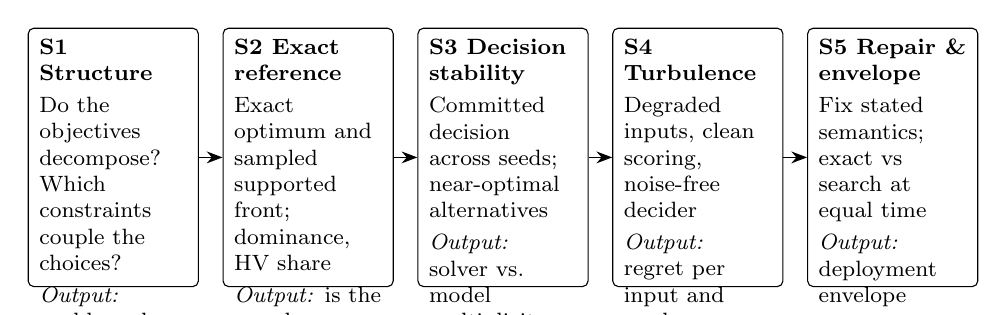
\begin{tikzpicture}[
  node distance=4mm and 3mm,
  auditbox/.style={draw, rounded corners=2pt, font=\footnotesize, inner sep=4pt,
    execute at begin node={\begin{minipage}[t][30mm][t]{0.155\textwidth}\raggedright},
    execute at end node={\end{minipage}}},
  arr/.style={-{Stealth[length=2mm]}, semithick}]
\node[auditbox] (s1) {\textbf{S1 Structure}\\[2pt] Do the objectives decompose? Which constraints couple the choices?\\[2pt] \emph{Output:} problem class};
\node[auditbox, right=of s1] (s2) {\textbf{S2 Exact reference}\\[2pt] Exact optimum and sampled supported front; dominance, HV share\\[2pt] \emph{Output:} is the search needed?};
\node[auditbox, right=of s2] (s3) {\textbf{S3 Decision stability}\\[2pt] Committed decision across seeds; near-optimal alternatives\\[2pt] \emph{Output:} solver vs.\ model multiplicity};
\node[auditbox, right=of s3] (s4) {\textbf{S4 Turbulence}\\[2pt] Degraded inputs, clean scoring, noise-free decider\\[2pt] \emph{Output:} regret per input and mode};
\node[auditbox, right=of s4] (s5) {\textbf{S5 Repair \& envelope}\\[2pt] Fix stated semantics; exact vs search at equal time\\[2pt] \emph{Output:} deployment envelope};
\draw[arr] (s1) -- (s2); \draw[arr] (s2) -- (s3); \draw[arr] (s3) -- (s4); \draw[arr] (s4) -- (s5);
\end{tikzpicture}
\caption{The five-step audit protocol for an optimisation-based decision system.\label{fig:protocol}}
\end{figure}

\subsection{S1 --- Structural check}
Write each objective as a function of the decision variables and ask whether it
decomposes. In the audited model every objective is a mean, over the directed people, of a
score that depends only on the person (ULPP) or on the person and the assigned centre (TIL,
CAIL); centre occupancy enters as an input that the allocation does not change, and there
is no capacity constraint. For non-negative weights $w$, the weighted sum
\begin{equation}
\sum_k w_k f_k(d) \;=\; \frac{1}{n_{\mathrm{dir}}}\sum_{j \text{ directed}}
\Bigl(w_1\,\mathrm{ULPP}_j + w_2\,\mathrm{TIL}_{j,c(j)} + w_3\,\mathrm{CAIL}_{j,c(j)}\Bigr)
\end{equation}
therefore separates by person: each person's best centre is independent of everyone
else's, and the optimum directs the $n_{\mathrm{dir}}$ people with the lowest best-case
cost. This greedy rule is exact, deterministic, and runs in $O(mn)$. S1 does not always end
the necessity question. When a constraint couples the choices, it names the problem class
instead (an assignment problem, a knapsack, a mixed-integer programme), and S2 then has to
show whether an exact method reaches the optimum at the target size (Section~\ref{sec:cases}).

\subsection{S2 --- Exact reference and dominance}
We compute the exact equal-weight optimum and a \emph{sampled supported reference front}: the
exact optima of the weighted sum on a regular lattice of the weight simplex (21 steps per
axis, 231 weight vectors). Every point of this front is exactly optimal for its weights, but
a finite lattice need not recover every supported non-dominated point, and unsupported points
are not sought at all~\cite{ehrgott2005multicriteria}; both omissions can only enlarge the true
front. Each front returned by the evolutionary system is compared with the exact optimum (how
many of its points the single exact point dominates) and with the reference front
(hypervolume share, with a common reference point at $1.1\times$ the component-wise maximum
over all fronts compared). Section~\ref{sec:rq1} reports how both quantities change when the
lattice is refined to 161 steps per axis.

\subsection{S3 --- Decision stability}
The published system returns a front and leaves the final choice to the user; to audit a
committed decision we fix a rule, the front point minimising the equal-weight,
min--max-normalised objective sum. A rule that ignores the front's extent (nearest to the
ideal point in raw objectives) gives the same seed floor ($0.83$ and $0.94$ against $0.83$
and $0.94$), so the floor is not an artefact of the rule. We solve the clean instance under 20 seeds
($1000 + 7919k$, $k = 0,\dots,19$) and compare the committed decisions of every seed pair
(190 pairs), with allocation churn, directed-set Jaccard and clean quality as defined in
Section~\ref{sec:model}. Confidence intervals for pairwise statistics are cluster-bootstrapped
over seeds, because pairs share seeds. Repeating this at $150$--$9600$ generations gives the
budget curve: decision quality and stability against compute.

The \emph{seed floor}, the mean churn between seeds, has three possible sources, and S3
separates them. The solver may stop far from the optimum, at a point that depends on the
seed. The model may admit many allocations of almost equal quality, so that even good
solvers disagree. And the rule that selects among equally good allocations may be unstated,
so that an exact solver returns whichever optimal vertex it reaches first. For the second
source we measure the multiplicity of the model directly, by modelling to generate
alternatives~\cite{brill1982mga}: for a tolerance $\varepsilon$ in objective-sum units, we
solve
\begin{equation}
\min_{d}\; \sum_{(j,i) \in P} d_{j,i}
\quad\text{s.t.}\quad d \text{ feasible},\quad F(d) \le F^\ast + \varepsilon,
\label{eq:mga}
\end{equation}
where $F$ is the equal-weight objective sum, $F^\ast$ its exact optimum and $P$ the
(person, centre) pairs of the allocations found so far, starting with the optimum. Each
solution is the allocation within $\varepsilon$ of the optimum that shares the fewest pairs
with the pool; five are generated per $\varepsilon$, and a variant that counts shared
directed people instead of shared pairs gives the smallest Jaccard index. Both are
mixed-integer programmes with binary $d$ (Appendix~\ref{app:mip}), solved by HiGHS under a
60\,s limit; 415 of the 420 solves were proven optimal, and the other five stopped within a
0.5\% gap, so the churn they report is a lower bound. We use $\varepsilon \in \{0, 0.1, 0.5, 1, 2, 5\}$ and
the evolutionary system's own quality deficit, so that the seed floor can be read against the
multiplicity of the model at the same quality. For the third source, the exact decider
commits through a stated tie-breaking rule: among allocations within $10^{-6}$ of $F^\ast$, it
returns the one with the smallest total weight under a fixed key, one pseudo-random weight in
$[1, 2)$ per (person, centre) pair from a published generator seed. A second lexicographic
solve computes it. Index-based keys would not suffice, because exchanging two people between
two centres leaves any sum of indices unchanged.

\subsection{S4 --- Input turbulence on a noise-free decider}
Turbulence perturbs one raw input field at a time in one of four modes: additive Gaussian
noise with standard deviation a fraction of the field's range, systematic bias, missing
entries imputed with the instance median or mode, and flips of categorical status. Levels
are $0.05, 0.1, 0.2, 0.4$ (fractions of the field's range for noise and bias, probabilities
for missing values and flips); every perturbed value is clipped to its valid range, and a level
$0$ run serves as an identity check. The levels are a sensitivity grid, not estimates of
real error rates: the empirical evidence we found~\cite{dehoratius2008inventory,altay2014haiti}
establishes that operational records are often wrong, but not by how much per field. Besides
the eight single-field cells we perturb with systematic bias in both directions, and with
three joint perturbations applied together at the same level: noise on all four continuous
fields; the transport triple (travel-duration noise, road-condition and hazard flips); and all
eight single-field cells at once. A decision is \emph{made} on degraded data and \emph{scored}
on the clean data. For a deterministic decider the difference between the two decisions' clean
scores is pure input sensitivity; for the exact decider it is the \emph{regret} of deciding on
degraded data, non-negative by construction. For the stochastic system the same difference
mixes input sensitivity with the seed floor of S3, so we report it above that floor
(Section~\ref{sec:model}). Trends over levels use a one-sided Spearman test with realisations
as units, levels $0.05$--$0.4$ only (level $0$ would add zeros by construction), and Holm
correction across cells. To test generalisation, the exact-decider study is repeated on five
further generated instances per size, under three demand conditions ($n_{\mathrm{dir}} = m/6$,
$m/3$, $m/2$) and two occupancy conditions (as generated, and every centre's occupancy raised
by 25 points).

\subsection{S5 --- Repair and deployment envelope}
If S1 shows that the model cannot express a property its documentation claims, repair the
model minimally and re-run S2. Here the claim is that CAIL penalises concentrating load on
stressed centres; the repair makes occupancy endogenous,
\begin{equation}
\mathrm{COR}'_i(\ell_i) = \min\Bigl(100,\; \mathrm{COR}_i + 100\,\frac{\ell_i}{\mathrm{cap}_i}\Bigr),
\qquad
\mathrm{CAIL}_{j,i} = \mathrm{FIS}_3\bigl(\mathrm{COR}'_i(\ell_i),\, \mathrm{RDR}_i,\, \mathrm{TD}_{j,i}\bigr),
\label{eq:repair}
\end{equation}
where $\ell_i$ is the number of people the decision sends to centre $i$ and
$\mathrm{cap}_i$ its capacity in persons, so that $\ell_i/\mathrm{cap}_i$ is the share of the
centre the decision fills; the symbols are defined in Section~\ref{sec:model}. This is the
definition of an occupancy rate, not a modelling choice, but the finding it leads to could
depend on it, so Section~\ref{sec:rq4} repeats the analysis with the load counted double, with
convex and concave forms $100(\ell_i/\mathrm{cap}_i)^{\gamma}$, $\gamma \in \{2, 0.5\}$, and with
the rule base's response to load tripled. Capacity is soft (faithful to the published semantics,
with an overload diagnostic) or hard (a constraint). The repaired model is no longer separable;
we solve it exactly as a mixed-integer programme in which only the load level of each centre is
binary (Appendix~\ref{app:mip}), with HiGHS~\cite{huangfu2018highs} through
SciPy~\cite{virtanen2020scipy}.

The envelope compares, on three generated instances per size from $150$ people and $5$ centres
to $3000$ people and $50$ centres, every method on the same instances and under the same
wall-clock limit ($60$\,s, and $300$\,s from $1000$ people up): the soft- and hard-capacity MIP;
NSGA-II stopped by a wall-clock deadline; NSGA-II whose initial population is seeded with the
deterministic fallback and the exact optima of the published model at 21 weight vectors; a
capacity-aware local search on the repaired model (best-improvement re-route and swap moves,
evaluated exactly from the per-load CAIL tables, started from the fallback or, with hard
capacity, from a capacity-respecting greedy allocation); and the deterministic fallback, the
exact optimum of the published model re-scored in the repaired one. Shared preparation is timed
separately: the fuzzy scores, needed by every method, and the CAIL-per-load tables, needed by
every method that sees the load. Each method is reported with its solver time and its total
decision latency, preparation included, and with its overload; all methods use the compiled
fuzzy evaluator. An instance on which the MIP finds no incumbent within the limit counts as
unsolved and is reported as such, never averaged. The submitted version calibrated the
generations of NSGA-II from a short timed run instead, and under its $300$\,s limit NSGA-II ran
between $183$ and $308$\,s; the deadline removes that imbalance.

\subsection{Software and reproducibility}
All steps run on the open reference implementation (Python 3.12.13, NumPy 2.4.4, SciPy
1.17.1, DEAP 1.4.3, pymoo 0.6.2, scikit-fuzzy 0.5.0) on an Apple M4 under macOS 15.8; every
manifest records this fingerprint. Hypervolume is computed with pymoo's exact indicator. A
compiled evaluator reproduces the
scikit-fuzzy inference to $10^{-9}$ and is pinned to it by tests; the exact greedy and the
MIP, the near-optimal alternatives and the tie-breaking rule are verified against brute-force
enumeration on small instances, and the local search's incremental bookkeeping against the
shared evaluator. Every run writes a manifest with seeds,
budgets, instance hash and environment fingerprint; the instances of the envelope are stored
with their SHA-256 hashes, and the data and code are archived with a DOI (Data Availability
Statement).

% =====================================================================
\section{Results}\label{sec:results}

\subsection{RQ1 --- Necessity}\label{sec:rq1}
The structural check (S1) is decisive on its own: every objective of the published model
is a mean of per-person or per-(person, centre) scores, so the exact optimum of any
weighted sum is the greedy rule of Section~\ref{sec:protocol}. Excluding the fuzzy
pre-computation that both methods share ($0.05$--$0.22$\,s with the compiled evaluator,
$4$--$16$\,s with scikit-fuzzy), it runs in
about $0.01$--$0.02$\,ms on the reference instances, against seconds for one evolutionary
solve.
The equal-weight optimum has an objective sum of $74.58$ on the small instance and $85.18$
on the large one; the weight sweep yields a sampled supported reference front of $181$ and
$197$ points.

The same check exposes a second mismatch between the model's equations and its
documentation, beside the one in CAIL that S5 repairs. The documentation reads a low mean ULPP
as ``directing the most vulnerable people''~\cite{rabiei2026resilient}. The rule base does the
opposite: FIS$_1$ assigns the highest ULPP to people who are highly vulnerable, live where
damage is severe and have little resource time left (Section~\ref{sec:model}), and the
objective minimises the mean ULPP over the people who are directed. ULPP and the crisp
priority score agree in rank ($\rho = 0.61$ small, $0.64$ large), so the exact optimum of the
published model directs the people of \emph{lowest} priority it can. Of the $n_{\mathrm{dir}}$
people the crisp rule ranks highest, the optimum directs $12\%$ (small) and $7\%$ (large); the
people it directs live with less damage than average ($44$ against $60$ on the $0$--$100$ scale,
small) and have more resource time left ($33$ against $25$\,h). Solving the reading the
documentation states, with ULPP replaced by $100 - \mathrm{ULPP}$, directs an almost disjoint
set ($8\%$ and $2\%$ overlap with the published optimum). The rest of the documentation shows
where the error lies: it defines ULPP as the unfairness of leaving a person out (if a person
who should be directed first is not, the score rises~\cite{rabiei2026resilient}). The rule base
follows that definition; the objective sums the score over the wrong set. Summed over the people
left out, as the definition requires, it is minimised by the same allocation as the mean of
$100 - \mathrm{ULPP}$ over the people directed, because $n_{\mathrm{dir}}$ is fixed. The evolutionary system optimises the
same objective and inherits the same preference, so the mismatch is a property of the model,
not of the solver. It also accounts for most of the gap between the crisp rule and the
optimum: on the small instance, $32$ of the $40$ units come from ULPP. We report the finding
here because S1 produced it. All results below concern the model as published. The corrected
reading changes which people are directed but not the structure RQ1 rests on, since
$100 - \mathrm{ULPP}_j$ is again a per-person score and the model stays separable; we have not
re-run RQ2--RQ4 under it.

Table~\ref{tab:rq1} compares this reference with the fronts the evolutionary system
returns. At the operational budget (150 generations, the artefact's default, against 200 in the
published experiments of~\cite{rabiei2026resilient}; the budget curve to 9600 generations makes the
choice immaterial for the conclusions), the
single exact optimum dominates every point of every front: $2000$ of $2000$ points over
20 seeds at both sizes. The fronts cover $39\%$ (small) and $21\%$ (large) of the reference
front's hypervolume, and their best point is $17.8$ and $33.3$ objective units worse than the
exact optimum. Figure~\ref{fig:fronts} shows the gap in two projections.
More compute narrows it without closing it: at $9600$ generations, sixty-four times the
operational budget, the exact point still dominates $32\%$ (small) and $97\%$ (large) of
front points, and the hypervolume share reaches $0.81$ and $0.42$.

The gap is not specific to one solver, population size or instance. NRGA and NSGA-III
match NSGA-II at the operational budget; at $2400$ generations NRGA comes closest of the
three (best front point $76.16$ against $74.58$) but still covers only $65\%$ of the reference
hypervolume. Spending the same $240{,}000$ evaluations on a larger population (200 or 400)
instead of more generations changes the hypervolume share by at most $0.03$. On two further
generated instances per size the exact optimum dominates $82$--$100\%$ of front points.
The published experiments of~\cite{rabiei2026resilient} pass through the same check
(Table~\ref{tab:paperA}): across three sizes, both model variants, three algorithms and
thirty repetitions, one deterministic point dominates $97$--$100\%$ of all front points.

The reference front is a sample, and refining it does not change these comparisons.
Table~\ref{tab:grid} solves the weighted sum on lattices of $21$ to $161$ steps per axis. The
number of supported points grows from $181$ to $1443$ (small) and from $197$ to $3359$ (large),
so the $21$-step lattice recovers only a fraction of them, but the front's hypervolume changes
by at most $1.1\%$ and the evolutionary fronts' share by at most $0.01$.

\begin{table}[H]
\centering
\caption{RQ1: the evolutionary system against the exact reference, $20$ seeds per row.
Dominated: front points dominated by the single exact equal-weight optimum, summed over seeds. HV
share: front hypervolume as a fraction of the sampled reference front's, mean and 95\% bootstrap
interval over seeds. Best: lowest objective sum on any front point. Churn: seed floor of the
committed decision with 95\% cluster-bootstrap interval. Exact optimum: small $74.58$, large
$85.18$; alternate instances $110.38$, $83.04$ (small) and $68.00$, $88.36$ (large).\label{tab:rq1}}
\footnotesize
\setlength{\tabcolsep}{4pt}
\begin{tabular}{llrlrl}
\toprule
Instance & Solver, budget & Dominated & HV share & Best & Churn\\
\midrule
Small & NSGA-II, 150 gen. & 2000/2000 & 0.39 [0.39, 0.40] & 92.39 & 0.83 [0.82, 0.85]\\
Small & NSGA-II, 2400 gen. & 1004/2000 & 0.72 [0.70, 0.73] & 79.55 & 0.61 [0.58, 0.64]\\
Small & NSGA-II, 9600 gen. & 630/2000 & 0.81 [0.80, 0.82] & 77.35 & 0.50 [0.47, 0.54]\\
Small & NRGA, 150 gen. & 1929/1929 & 0.36 [0.35, 0.38] & 92.26 & 0.85 [0.83, 0.86]\\
Small & NRGA, 2400 gen. & 356/2000 & 0.65 [0.64, 0.66] & 76.16 & 0.39 [0.36, 0.41]\\
Small & NSGA-III, 150 gen. & 1996/1996 & 0.40 [0.38, 0.42] & 91.10 & 0.83 [0.81, 0.85]\\
Small & NSGA-III, 2400 gen. & 871/2000 & 0.72 [0.69, 0.74] & 77.11 & 0.55 [0.49, 0.62]\\
Small & NSGA-II, $\mu=200$, 240k eval. & 1851/4000 & 0.73 [0.71, 0.75] & 76.97 & 0.61 [0.56, 0.66]\\
Small & NSGA-II, $\mu=400$, 240k eval. & 5039/8000 & 0.69 [0.67, 0.71] & 77.71 & 0.64 [0.60, 0.68]\\
Large & NSGA-II, 150 gen. & 2000/2000 & 0.21 [0.21, 0.22] & 118.46 & 0.94 [0.93, 0.95]\\
Large & NSGA-II, 2400 gen. & 2000/2000 & 0.37 [0.37, 0.38] & 110.03 & 0.91 [0.90, 0.91]\\
Large & NSGA-II, 9600 gen. & 1945/2000 & 0.42 [0.41, 0.43] & 105.71 & 0.90 [0.88, 0.91]\\
\midrule
Small, alt.\ 1 & NSGA-II, 150 gen. & 1630/2000 & 0.45 [0.44, 0.46] & 125.16 & 0.86 [0.84, 0.87]\\
Small, alt.\ 2 & NSGA-II, 150 gen. & 1968/2000 & 0.41 [0.40, 0.43] & 95.58 & 0.78 [0.76, 0.80]\\
Large, alt.\ 1 & NSGA-II, 150 gen. & 1976/1976 & 0.16 [0.16, 0.17] & 106.20 & 0.94 [0.94, 0.95]\\
Large, alt.\ 2 & NSGA-II, 150 gen. & 2000/2000 & 0.17 [0.16, 0.17] & 120.27 & 0.95 [0.95, 0.96]\\
\bottomrule
\end{tabular}
\end{table}

\begin{figure}[H]
\centering
\includegraphics[width=\textwidth]{fig2_fronts_vs_exact.pdf}
\caption{Fronts of the evolutionary system (one seed each, 150 and 2400 generations) against
the exact supported front and the exact equal-weight optimum, small instance, in two
projections of the three-objective space. Lower is better on every axis.\label{fig:fronts}}
\end{figure}

\begin{table}[H]
\centering
\caption{The published experiments of~\cite{rabiei2026resilient} (30 repetitions, population
100, 200 generations) through the S2 dominance check: front points dominated by the single
exact equal-weight optimum.\label{tab:paperA}}
\small
\begin{tabular}{llrrrrr}
\toprule
Size & Model & Exact sum & NSGA-II & NRGA & NSGA-III & Best MOEA sum\\
\midrule
Small & 3-obj. & 74.58 & 2976/2994 & 2838/2838 & 3000/3000 & 84.20\\
Small & 4-obj. & 112.03 & 2950/3000 & 2883/2973 & 2948/3000 & 129.75\\
Medium & 3-obj. & 68.76 & 3000/3000 & 2908/2908 & 3000/3000 & 94.71\\
Medium & 4-obj. & 105.31 & 2996/3000 & 2997/2997 & 2996/3000 & 136.71\\
Large & 3-obj. & 85.18 & 3000/3000 & 2781/2781 & 3000/3000 & 116.24\\
Large & 4-obj. & 121.87 & 2997/3000 & 2994/2994 & 2993/3000 & 158.91\\
\bottomrule
\end{tabular}
\end{table}

\begin{table}[H]
\centering
\caption{Sensitivity of the sampled supported reference front to the weight lattice. HV: the
front's hypervolume relative to the 161-step front (common reference point). Share: hypervolume
of the evolutionary fronts at 150 and 9600 generations as a fraction of the reference front's,
mean over seeds. Steps per axis of the weight lattice; S, L: small, large. One reference point per
instance, $1.1\times$ the maximum over the finest front and all evolutionary fronts, serves all
lattices, so the shares are slightly below those of Table~\ref{tab:rq1}.\label{tab:grid}}
\footnotesize
\begin{tabular}{rrrcccc}
\toprule
& & & \multicolumn{2}{c}{Small} & \multicolumn{2}{c}{Large}\\
\cmidrule(lr){4-5}\cmidrule(lr){6-7}
Steps & Vectors & Points (S / L) & HV & Share 150 / 9600 & HV & Share 150 / 9600\\
\midrule
21 & 231 & 181 / 197 & 0.989 & 0.365 / 0.805 & 0.994 & 0.160 / 0.351\\
41 & 861 & 480 / 647 & 0.996 & 0.363 / 0.799 & 0.998 & 0.160 / 0.350\\
81 & 3321 & 994 / 1736 & 0.999 & 0.362 / 0.797 & 0.999 & 0.160 / 0.349\\
161 & 13041 & 1443 / 3359 & 1.000 & 0.361 / 0.796 & 1.000 & 0.159 / 0.349\\
\bottomrule
\end{tabular}
\end{table}

The answer to RQ1 is no. For the model as published, the evolutionary search is not needed,
and at every budget we tested it returns allocations that a deterministic rule improves on
in every objective at once.

\subsection{RQ2 --- Decision stability}\label{sec:rq2}
Reproducibility holds, and across platforms: the same seed reproduces the same front bit
for bit within one environment, a decision recomputed from a stored front matched the
original run exactly, and a continuous-integration matrix (macOS arm64 and Ubuntu x86-64,
Python 3.11 and 3.12) produced identical front signatures for all ten (instance, seed)
combinations at the operational budget (Appendix~\ref{app:crossenv}). Decision stability does not.
Two runs on identical clean data with different seeds commit to allocations that differ for
$83.4\%$ [$82.0$, $84.7$] of the directed people on the small instance and $93.9\%$ [$93.3$,
$94.5$] on the large one (190 seed pairs each, cluster-bootstrap 95\% CI). The directed sets
overlap by a Jaccard index of only $0.31$ and $0.25$: most of the people one run chooses to
direct, the other run does not direct at all. The committed decisions also differ in quality,
with a standard deviation of $2.05$ (range $92.4$--$101.6$) and $1.32$ objective units.

Figure~\ref{fig:budget} shows how this floor responds to compute. On the small instance it
falls from $0.83$ to $0.50$ between $150$ and $9600$ generations while quality improves
from $97.4$ to $81.1$, still short of the exact $74.58$; on the large instance it stays at
$0.90$ or above throughout. The other solvers and instances give the same picture at the
operational budget (churn $0.85$ for NRGA and $0.83$ for NSGA-III; $0.78$--$0.95$ on the
alternate instances, Table~\ref{tab:rq1}).

\begin{figure}[H]
\centering
\includegraphics[width=\textwidth]{fig3_budget_curve.pdf}
\caption{Budget curve. Top: clean quality of the committed decision (mean $\pm$ s.d.\ over
seeds) against the exact optimum. Bottom: allocation churn between committed decisions of
different seeds on identical clean data. Both sizes: 20 seeds at 150, 2400 and 9600 generations,
5 at the intermediate budgets. Dashed in the lower panels: the exact decider with the
tie-breaking rule of S3.\label{fig:budget}}
\end{figure}

How much of this floor is due to the solver, and how much to the model?
Figure~\ref{fig:multiplicity} answers with the near-optimal alternatives of
Eq.~(\ref{eq:mga}). Near the optimum the model is flat. Within $1$ objective unit of it, about
$1\%$ of the optimal value, there are allocations that differ from the optimum for $26\%$ of the
directed people (small) and $33\%$ (large); within $5$ units, for $62\%$ and $73\%$. At the
evolutionary system's own quality deficit, $17.8$ and $33.3$ units, the model admits
allocations that share no (person, centre) pair with the optimum, and directed sets whose
Jaccard index with the optimum's is $0.08$ and $0$. These are the most different allocations
within each tolerance, not typical ones; the mean churn among the five found is somewhat lower
($0.24$ against $0.26$ at $\varepsilon = 1$ on the small instance, $0.62$ against $0.73$ for the
large hard-capacity model). The repaired models are flatter still: with
hard capacity, allocations within one unit differ for $52\%$ (small) and $73\%$ (large) of the
people. The seed floor of $0.83$ and $0.94$ therefore sits in a region where the model itself
allows almost any allocation, and a solver that stops there has no reason to stop at the same
one twice. Solver non-convergence and model multiplicity are not alternatives here: the solver's
deficit is what exposes the multiplicity.

The exact decider removes the solver's part but not the model's. Its optimum is unique on the
small instance under all three models, but not on the large one: alternative optima differ
from the reported one for $1\%$ of the directed people in the published model, $6\%$ with soft
capacity and $22\%$ with hard capacity. Which of them a solver returns depends on details as
incidental as the order in which the people are listed. Presented with the same large instance
in ten random orders, the hard-capacity MIP returned ten different optimal allocations, and the
soft one nine (Table~\ref{tab:tiebreak}); this is the mechanism behind the two platforms of
Appendix~\ref{app:crossenv}. With the tie-breaking rule of S3 the exact decider committed to
one allocation in every cell. A floor of zero is thus a property of the decider together with
its selection policy, not of exactness alone.

\begin{table}[H]
\centering
\caption{The tie-breaking rule. Distinct optimal allocations returned when the same instance is
presented in ten random orders of the people; plain: HiGHS without a selection policy (the
published model: the greedy rule with ties to the lower index); canonical: with the
tie-breaking rule of S3.\label{tab:tiebreak}}
\small
\begin{tabular}{lcccccc}
\toprule
& \multicolumn{3}{c}{Small} & \multicolumn{3}{c}{Large}\\
\cmidrule(lr){2-4}\cmidrule(lr){5-7}
& Published & Soft $\kappa=2$ & Hard $\kappa_f=1.5$ & Published & Soft $\kappa=2$ & Hard $\kappa_f=1.5$\\
\midrule
Plain & 1 & 1 & 1 & 1 & 9 & 10\\
Canonical & 1 & 1 & 1 & 1 & 1 & 1\\
\bottomrule
\end{tabular}
\end{table}

\begin{figure}[H]
\centering
\includegraphics[width=\textwidth]{fig_multiplicity.pdf}
\caption{Multiplicity of the model near its optimum. Largest churn (left) and smallest
directed-set Jaccard index (right) against the optimum among allocations within $\varepsilon$
of it, for the published model and the two repaired variants; $\varepsilon$ as a share of the
optimal value. Markers: the seed floor of the evolutionary system, plotted at its quality
deficit.\label{fig:multiplicity}}
\end{figure}

The floor also explains our original turbulence result. Comparing a decision made on
degraded inputs with the clean decision \emph{for the same seed}, the evolutionary system
re-routed about $83\%$ of the people at the smallest perturbation and stayed there. That
plateau equals the seed floor in every cell we measured (difference at most $0.02$). A changed
input changes the fitness landscape, and a changed landscape decorrelates the search as
completely as a new seed does. Missing centre-occupancy values show the mechanism exactly:
a realisation that blanks no centre leaves the inputs unchanged and the churn at zero, while
one that blanks any centre jumps to the floor, and the fraction of realisations with at
least one blanked centre predicts the mean churn to within $0.003$ at every level.

Small quality differences do not make these decisions interchangeable. In relief, as in any
rationing of scarce supply, the allocation is a list of named recipients: who is directed,
and where, is what the people affected experience and what an operator must justify. Two
allocations of near-equal aggregate quality that direct different people are different
decisions with different winners. Instability alone does not make a decision illegitimate. A
documented randomised policy, a lottery among equally good allocations, can be fair and
accountable, and a deterministic rule can select arbitrarily. What the audit trail needs is a
stated policy for selecting among near-equivalent allocations. A seeded stochastic search
supplies none: its selection among the many allocations the model allows is a by-product of
the seed and the stopping point, which no one chose and no one can defend to the person who was
not directed. Running the system several times and committing to the consensus narrows the
spread but does not close it (Appendix~\ref{app:consensus}).

The answer to RQ2 is that the system is reproducible but its decision is not stable. Seed
pinning makes a run repeatable; it does not make its output \emph{the} decision, because the
next seed, equally valid, commits to a different allocation for most of the people. The
instability arises where the solver stops in a region in which the model admits many
near-equivalent allocations, and it is completed by the absence of a selection policy; the two
are not separable shares, since the floor falls as the solver converges (Figure~\ref{fig:budget}). An exact decider with a stated
tie-breaking rule addresses both: it commits at the optimum, where the model admits the fewest
alternatives, and chooses among tied optima by a rule that can be published and defended.

\subsection{RQ3 --- Input fragility}\label{sec:rq3}
With solver noise removed, input fragility becomes measurable. On the two reference instances,
over 50 realisations per level, the regret of the exact decider grows with the turbulence level
in all sixteen single-field cells (eight field/mode cells at two sizes; one-sided Spearman over
levels $0.05$--$0.4$, $\rho = 0.37$--$0.97$, Holm-adjusted $p < 10^{-6}$). It is small at the
lowest level (under $1$ objective unit) and reaches $5$--$8$ units at level $0.4$ for the
continuous inputs the objectives consume (travel duration, resource time, damage level, centre
occupancy), with the largest cell mean, $14.5$, for centre-occupancy noise on the large instance.

Table~\ref{tab:rq3} and Figure~\ref{fig:turbulence} test whether this holds beyond the reference
instances: six instances per size, three demand and two occupancy conditions, $36$ conditions in
all, with systematic bias and three joint perturbations added. It does. In every condition the
regret of every noise, missing-value and flip cell grows with the level (Holm-adjusted, all
$36 \times 8$ tests per size significant), and the ranking of the inputs is the one found on the
reference instances: the continuous inputs the objectives consume cost most, categorical flips
less, and median-imputed missing values least. Systematic bias of a given size costs about two
thirds as much as noise of the same size on resource time, between half and the full noise effect on
travel time, and half or less on damage and occupancy, in either direction; with one realisation and four levels per condition its
trend tests have little power, so we report its magnitude only. Occupancy perturbations vary most
between conditions; our reading is that their effect depends on how close the centres already are
to the occupancy breakpoints of FIS$_3$. Joint perturbations add up and do not amplify each other: at level $0.4$, perturbing all
eight cells at once costs $29$ (small) and $32$ (large) units, $0.78$--$0.79$ of the sum of its
single-field parts, and the transport triple costs $0.96$--$0.98$ of its parts. The joint
perturbations change most of the directed people at level $0.4$ (churn $0.59$--$0.86$); among
single fields, only occupancy noise on the large instances does ($0.61$).

\begin{table}[H]
\centering
\caption{RQ3 across $36$ conditions per size (six instances, three demand, two occupancy
conditions): regret of the exact decider, median over conditions of the per-condition mean, at
levels $0.05$ and $0.4$ with the range over conditions, and the median allocation churn at level
$0.4$. Joint rows: in parentheses, the regret as a share of the sum of the single-field regrets
in the same condition.\label{tab:rq3}}
\scriptsize
\setlength{\tabcolsep}{3pt}
\begin{tabular}{lrlrrlr}
\toprule
& \multicolumn{3}{c}{Small} & \multicolumn{3}{c}{Large}\\
\cmidrule(lr){2-4}\cmidrule(lr){5-7}
Field, mode & $0.05$ & $0.4$ [range] & churn & $0.05$ & $0.4$ [range] & churn\\
\midrule
Travel time, noise & 0.63 & 6.9 [4.4, 8.5] & 0.42 & 0.85 & 6.7 [5.2, 8.9] & 0.45\\
Resource time, noise & 0.33 & 7.4 [4.9, 9.8] & 0.32 & 0.35 & 7.5 [5.5, 10.2] & 0.32\\
Damage, noise & 0.20 & 5.1 [2.9, 8.2] & 0.28 & 0.22 & 5.7 [3.4, 8.5] & 0.28\\
Occupancy, noise & 0.28 & 6.3 [4.2, 10.9] & 0.43 & 0.46 & 9.2 [6.7, 14.6] & 0.61\\
Road, flip & 0.35 & 3.5 [2.8, 4.6] & 0.26 & 0.43 & 3.8 [3.4, 4.4] & 0.32\\
Hazard, flip & 0.26 & 2.3 [1.7, 3.2] & 0.22 & 0.29 & 2.8 [2.3, 3.2] & 0.26\\
Damage, missing & 0.17 & 1.6 [0.7, 3.8] & 0.13 & 0.19 & 1.5 [1.0, 3.6] & 0.11\\
Occupancy, missing & 0.04 & 0.5 [0.0, 7.3] & 0.09 & 0.04 & 1.9 [0.3, 3.9] & 0.23\\
\midrule
Travel time, bias $+$ & 0.60 & 4.5 [2.5, 7.3] & 0.38 & 0.78 & 6.6 [4.6, 10.1] & 0.54\\
Travel time, bias $-$ & 0.45 & 3.4 [1.6, 5.3] & 0.22 & 0.85 & 4.8 [2.8, 8.3] & 0.30\\
Resource time, bias $+$ & 0.13 & 5.0 [3.2, 8.3] & 0.32 & 0.16 & 5.3 [3.4, 8.7] & 0.34\\
Resource time, bias $-$ & 0.15 & 4.6 [2.9, 9.1] & 0.28 & 0.14 & 5.2 [3.1, 8.2] & 0.33\\
Damage, bias $+$ & 0.06 & 2.6 [1.1, 6.6] & 0.23 & 0.05 & 2.3 [1.3, 6.2] & 0.20\\
Damage, bias $-$ & 0.05 & 2.0 [0.9, 4.2] & 0.17 & 0.04 & 2.1 [1.3, 4.9] & 0.18\\
Occupancy, bias $+$ & 0.05 & 0.9 [0.0, 9.2] & 0.15 & 0.07 & 2.5 [0.8, 13.1] & 0.39\\
Occupancy, bias $-$ & 0.06 & 1.0 [0.1, 9.5] & 0.20 & 0.10 & 2.5 [0.0, 7.5] & 0.37\\
\midrule
Joint: continuous noise & 1.42 & 23.7 [17.3, 32.6] & 0.73 (0.91) & 1.91 & 26.3 [19.3, 34.0] & 0.81 (0.88)\\
Joint: transport & 1.41 & 12.3 [10.6, 14.1] & 0.59 (0.98) & 1.54 & 12.9 [11.8, 14.3] & 0.66 (0.96)\\
Joint: all eight & 2.40 & 28.8 [21.1, 38.8] & 0.76 (0.79) & 3.02 & 31.5 [23.9, 40.9] & 0.86 (0.78)\\
\bottomrule
\end{tabular}
\end{table}

\begin{figure}[H]
\centering
\includegraphics[width=\textwidth]{fig4_turbulence_regret.pdf}
\caption{Regret of the exact decider by field and perturbation mode at levels $0.05$, $0.1$ and
$0.4$: median over the $36$ conditions per size of the per-condition mean regret, with the
10th--90th percentile range over conditions.\label{fig:turbulence}}
\end{figure}

Two comparisons put these numbers in scale. First, the mean degraded exact decision in the worst
single-field cell of the small reference instance (travel-duration noise at level $0.4$, about
$82.6$; worst single realisation $86.9$) is still better than the evolutionary system's
\emph{clean} committed decision at the operational budget ($97.4$), and on a par with its clean
decision at $9600$ generations ($81.1$). Second, the crisp priority rule used as a
no-optimisation reference degrades by comparable amounts under centre-side and transport
perturbations, from a clean decision that is $40$ (small) and $44$ (large) units worse than the
exact optimum. Under person-side noise its loss in the published objectives can even be negative. The ULPP
finding of Section~\ref{sec:rq1} is consistent with this: the crisp rule directs the
highest-priority people, whom the published objective penalises, so noise that blurs its ranking
moves it towards people the objective rewards. For the evolutionary system (150 generations; 12 and 8
realisations per level, 8 and 6 seeds; all eight cells on the small instance and four on the
large one), the turbulence harm above its seed floor shows significant trends for travel-duration,
resource-time, damage-level and centre-occupancy noise and for damage-level missing values on the
small instance, and for centre-occupancy and damage-level noise and road-condition flips on the
large one, but it is buried under a decision-to-decision spread of the same size.

The answer to RQ3 is that the system's input fragility, measured in its own objectives, is real,
grows smoothly with the turbulence level and is concentrated in the inputs its objectives consume,
on every instance and condition we tested. At levels $0.05$--$0.1$ of single-field noise the regret
is at most $2.5$ units on the reference instances, an order of magnitude smaller than the cost of
the solver it was hidden behind ($22.8$ and $35.5$ units at the operational budget). Whether such
levels are realistic for a given field is an empirical question that the data we found do not
answer.

\subsection{RQ4 --- Repair and deployment envelope}\label{sec:rq4}
The documentation of the audited system states that CAIL is low when load is spread and
rises when a decision piles people onto stressed centres~\cite{rabiei2026resilient}. The
published equations cannot express that: occupancy enters CAIL as a fixed input, so the
exact optimum sends $38$ of $50$ people to one centre on the small instance and $69$ of
$100$ on the large one. The repair of Section~\ref{sec:protocol} makes occupancy depend on
the assigned load, either softly (the objective sees the load; an overload diagnostic counts
people beyond free capacity) or with a hard capacity limit. We vary the capacity scale:
$\kappa$ sets centre size to $\lceil\kappa\, n_{\mathrm{dir}}/n\rceil$ in the soft variant
($\kappa = \infty$ recovers the published model), and $\kappa_f$ sets total free places to
$\kappa_f\, n_{\mathrm{dir}}$ in the hard one.

Table~\ref{tab:rq4} gives three results. First, the soft repair restores the intended
direction but not its strength: on the large instance the optimum now spreads load over more
centres and the published optimum becomes $11$--$12\%$ worse, yet on the small instance the
published optimum stays within $1.5\%$ and overload persists at every $\kappa$. Second, a hard
capacity limit is what makes the optimum physically feasible; the published optimum violates it
by $14$--$50$ people, and the feasible optimum differs from that infeasible decision by $-4.3$ to
$+6.4$ objective units. Third, every repaired variant is still solved to proven optimality in at
most $3.7$\,s.

\begin{table}[H]
\centering
\caption{RQ4: the repaired model solved exactly. Quality: objective sum of the MIP optimum
(repaired model). Max load: people at the busiest centre. Overload: people beyond free
capacity. Published-optimum columns: the exact optimum of the published (separable) model,
re-scored in the repaired model. All MIP solves proven optimal (gap $\le 10^{-4}$).\label{tab:rq4}}
\small
\begin{tabular}{llrrrrrr}
\toprule
& & \multicolumn{4}{c}{MIP optimum, repaired model} & \multicolumn{2}{c}{Published optimum}\\
\cmidrule(lr){3-6}\cmidrule(lr){7-8}
Size & Capacity & Quality & Max load & Overload & Time (s) & Quality & Overload\\
\midrule
Small & soft, $\kappa=\infty$ & 74.58 & 38 & 0.0 & 0.01 & 74.58 & 0.0\\
Small & soft, $\kappa=1$ & 110.15 & 41 & 33.2 & 0.42 & 111.33 & 30.2\\
Small & soft, $\kappa=2$ & 107.08 & 36 & 20.5 & 0.53 & 108.23 & 22.5\\
Small & soft, $\kappa=3$ & 104.85 & 32 & 8.7 & 1.38 & 106.45 & 14.7\\
Small & hard, $\kappa_f=1.2$ & 114.95 & 14 & 0 & 0.07 & 108.52 & 23.5\\
Small & hard, $\kappa_f=1.5$ & 110.95 & 18 & 0 & 0.54 & 107.53 & 19.9\\
Small & hard, $\kappa_f=2$ & 105.79 & 24 & 0 & 0.18 & 106.35 & 13.9\\
\midrule
Large & soft, $\kappa=\infty$ & 85.18 & 69 & 0.0 & 0.07 & 85.18 & 0.0\\
Large & soft, $\kappa=1$ & 100.89 & 41 & 83.7 & 0.82 & 111.84 & 80.2\\
Large & soft, $\kappa=2$ & 100.26 & 43 & 77.8 & 0.84 & 111.70 & 63.3\\
Large & soft, $\kappa=3$ & 99.71 & 40 & 68.6 & 0.89 & 111.66 & 50.6\\
Large & hard, $\kappa_f=1.2$ & 113.90 & 24 & 0 & 0.84 & 111.65 & 49.9\\
Large & hard, $\kappa_f=1.5$ & 109.07 & 23 & 0 & 0.35 & 111.63 & 45.1\\
Large & hard, $\kappa_f=2$ & 105.27 & 31 & 0 & 3.67 & 109.52 & 37.1\\
\bottomrule
\end{tabular}
\end{table}

Is the first result an artefact of the repair's linear form? Table~\ref{tab:forms} repeats the
grid under four alternatives: the load counted double, convex and concave shares, and the
published rule base with its response to load tripled. Every solve is again proven optimal, in
at most $11.4$\,s. The convex form, under which light loads matter little and heavy loads a lot,
spreads load most and is the only one that removes overload in one cell. Tripling the rule base's
response makes the published optimum up to $46\%$ worse in the repaired model, so the objective
now separates good from bad allocations far more sharply, but the soft optimum still overloads
centres by $18$--$92$ people. The explanation in the submitted version, a rule base with too little
dynamic range, is therefore only part of it. The binding limit is that CAIL saturates once a
centre is full: beyond that point the soft objective is indifferent to further load, whatever the
range below it. Under every form we tested, only the hard constraint removed overload.

\begin{table}[H]
\centering
\caption{Sensitivity of RQ4 to the form of the repair: soft capacity, $\kappa \in \{1, 2, 3\}$,
range over the three values. Overload: people beyond free capacity in the MIP optimum. Penalty:
how much worse the published optimum is in the repaired model. All solves proven
optimal.\label{tab:forms}}
\small
\begin{tabular}{llrrrr}
\toprule
& & \multicolumn{2}{c}{Small} & \multicolumn{2}{c}{Large}\\
\cmidrule(lr){3-4}\cmidrule(lr){5-6}
Form & $\mathrm{COR}'_i$ & Overload & Penalty & Overload & Penalty\\
\midrule
Linear (paper) & $\mathrm{COR}_i + 100\,\ell_i/\mathrm{cap}_i$ & 8.7--33.2 & 1.1--1.5\% & 68.6--83.7 & 10.9--12.0\%\\
Amplified & $\mathrm{COR}_i + 200\,\ell_i/\mathrm{cap}_i$ & 14.7--32.5 & 0.2--1.1\% & 72.5--85.7 & 10.9--11.1\%\\
Convex & $\mathrm{COR}_i + 100\,(\ell_i/\mathrm{cap}_i)^2$ & 0.0--30.2 & 1.9--12.9\% & 57.6--82.9 & 11.7--14.6\%\\
Concave & $\mathrm{COR}_i + 100\,(\ell_i/\mathrm{cap}_i)^{1/2}$ & 14.7--27.5 & 0.2--0.6\% & 67.6--85.7 & 10.7--10.8\%\\
Stretched rule base & linear; load response $\times 3$ & 17.8--33.7 & 5.9--10.5\% & 76.6--91.9 & 45.4--46.1\%\\
\bottomrule
\end{tabular}
\end{table}

The envelope extends the comparison to larger generated instances, from $150\times5$ to
$3000\times50$ people $\times$ centres with one third of the people directed, three instances per
size (Table~\ref{tab:envelope}, Figure~\ref{fig:scaling}, per instance in
Appendix~\ref{app:envelope}). Every method runs on the same instances under the same wall-clock
limit, and Table~\ref{tab:envelope} reports total decision latency next to solver time.

\begin{table}[H]
\centering
\caption{Deployment envelope on the repaired model, three instances per size; every method on the same instances. Soft capacity ($\kappa=2$): quality and overload (people beyond free capacity) in the soft model. Hard capacity ($\kappa_f=1.5$): quality in the hard model. Means over solved instances; $s/p$: instances with an incumbent / proven optimal. LS: local search; seeded: NSGA-II seeded with exact solutions of the published model; fallback: exact optimum of the published model. Latency: total decision time of the hard-capacity local search, preparation of scores and load table included (s).\label{tab:envelope}}
\scriptsize
\setlength{\tabcolsep}{3pt}
\resizebox{\textwidth}{!}{%
\begin{tabular}{lr|rcrrrrr|rcrr}
\toprule
& & \multicolumn{7}{c|}{Soft capacity} & \multicolumn{4}{c}{Hard capacity}\\
Size & Limit & MIP & $s/p$ & LS & NSGA-II & Seeded & Fallback & Overload$^\ast$ & MIP & $s/p$ & LS & Latency\\
\midrule
$150\times5$ & 60\,s & 110.2 & 3/3 & 110.4 & 116.8 & 116.5 & 112.4 & 27/25/25/34/25 & 114.2 & 3/3 & 115.6 & 1\\
$300\times10$ & 60\,s & 100.5 & 3/3 & 100.6 & 121.6 & 109.9 & 107.2 & 67/65/45/63/67 & 106.6 & 3/3 & 108.1 & 3\\
$600\times20$ & 60\,s & 97.3 & 3/3 & 97.7 & 129.7 & 101.1 & 102.1 & 138/126/65/124/146 & 102.4 & 3/3 & 103.9 & 11\\
$1000\times25$ & 60\,s & 96.6 & 3/1 & 97.1 & 133.6 & 102.0 & 102.8 & 243/227/111/218/242 & 102.5 & 3/3 & 103.6 & 28\\
$1500\times40$ & 60\,s & 98.8 & 3/0 & 96.5 & 139.8 & 99.3 & 100.3 & 413/365/149/362/404 & 103.8 & 3/3 & 105.0 & 65\\
$3000\times50$ & 60\,s & 150.7 & 1/0 & 95.7 & 143.1 & 99.0 & 99.7 & 869/753/329/744/800 & -- & 0/0 & 103.6 & 172\\
\midrule
$1000\times25$ & 300\,s & 96.6 & 3/3 & 97.1 & 130.5 & 102.0 & 102.8 & 242/227/108/218/242 & 102.5 & 3/3 & 103.6 & 29\\
$1500\times40$ & 300\,s & 95.7 & 3/1 & 96.5 & 136.6 & 99.9 & 100.3 & 383/365/147/376/404 & 103.8 & 3/3 & 105.0 & 60\\
$3000\times50$ & 300\,s & 96.5 & 3/0 & 95.7 & 139.6 & 99.1 & 99.7 & 845/753/339/770/800 & 102.7 & 3/1 & 103.6 & 178\\
\bottomrule
\multicolumn{13}{l}{$^\ast$ Overload of MIP / LS / NSGA-II / seeded / fallback, soft model. Hard-capacity methods have zero overload by construction.}\\
\end{tabular}}
\end{table}


Up to $600\times20$ both MIPs are proven optimal within a minute, and the capacity-aware local
search, started from the fallback, comes within $0.2$--$0.5$ units of the soft optimum in under a
second of solver time. At $1000\times25$ and beyond the picture changes. The soft MIP proves
optimality on all three instances at $1000\times25$ only with five minutes, on one of three at
$1500\times40$, and on none at $3000\times50$, where under one minute it finds an incumbent on
one instance only. The hard MIP proves optimality up to $1500\times40$ within a minute; at
$3000\times50$ it finds nothing within a minute and proves optimality on one of three instances
within five, with gaps of about $0.02\%$ on the others. Under the one-minute limit the local
search returns better soft-capacity allocations than the MIP from $1500\times40$ on ($96.5$
against $98.8$; at $3000\times50$, $95.7$ on all three instances against one solved instance).
With five minutes the MIP overtakes it at $1500\times40$ ($95.7$ against $96.5$) but not at
$3000\times50$ ($96.5$ against $95.7$), and the local search needs under $17$\,s of solver time
throughout. With hard capacity it stays within $1.5\%$ of the MIP on average at every size while
needing under $4$\,s of solver time; the hard MIP at $3000\times50$ needs $115$\,s on the instance it
proves and reaches the limit on the other two.

The evolutionary system does not take this regime. Given the same wall-clock time, it is
$6$--$43$ units behind the soft MIP wherever the MIP proved optimality or came within a few
per cent of it, ahead of the one-minute MIP only at $3000\times50$, where the MIP found a single
poor incumbent, and behind the deterministic fallback at every size. Its allocations overload the
centres least of all the soft-capacity methods (Appendix~\ref{app:envelope}), because they spread
people almost at random, at a cost of up to $43$ units in quality. Seeding its population with exact solutions of the
published model helps, by up to $44$ units from $300\times10$ on, but the seeded search stays
close to its seeds: from $600\times20$ on it ends within about $1$ unit of the fallback, it stays
behind the local search, and it inherits the fallback's overload. Preparation dominates the
latency at scale. At $3000\times50$ the fuzzy scores take about $10$\,s and the CAIL-per-load
tables about $95$\,s (soft) and $160$\,s (hard), so the total latency of the hard-capacity local
search is about $3$\,min although its search takes $3$\,s; any method that sees the load pays this
cost, and only the fallback, which does not, decides in about $10$\,s.

\begin{figure}[H]
\centering
\includegraphics[width=\textwidth]{fig5_scaling.pdf}
\caption{Deployment envelope: quality in the soft repaired model, mean over the solved instances
of each size, at the $60$\,s (left) and $300$\,s (right) limits. Annotations mark sizes with
instances on which the MIP found no incumbent.\label{fig:scaling}}
\end{figure}

The answer to RQ4 is that the repair changes what the optimum looks like but not who should
compute it at the sizes the system targets: there, exact optimisation is fast and strictly
better. Beyond them, a capacity-aware local search is the better tool under tight time limits,
and close to the MIP under looser ones, with the exact decider of
the published model as its starting point; the audited evolutionary system, seeded or not, is
not competitive at any size we tested.

\subsection{The protocol on two further models}\label{sec:cases}
For the relief model S1 settled necessity at once. Two further models show what the protocol
does when it does not. Both are audited with S1--S3 under the same settings (population $100$,
$20$ seeds, the committal rule of Eq.~(\ref{eq:committal})); Table~\ref{tab:cases} reports them.

The first is the ED volunteer-staffing model from which the relief tool
grew~\cite{rabiei2023volunteer}, still our own but built differently: every emergency department
posts one vacancy of one skill type, each vacancy must be filled by exactly one volunteer of that
type, no volunteer fills two, and two fuzzy objectives (mean importance of unmet needs, mean
preference dissatisfaction) are minimised with NSGA-II or NRGA over a permutation encoding. S1
finds that the one-to-one constraint couples the choices, so the model is not separable. It also
names the problem class: every weighted sum is a rectangular linear assignment problem, solved
exactly in polynomial time~\cite{kuhn1955hungarian}. The instances come from the artefact's
deterministic benchmark generator. On the small instance ($75$ volunteers,
$5$ vacancies) the evolutionary system comes close: averaged over seeds, its best front point is
$0.2\%$ above the exact equal-weight optimum, and $11$ of $20$ NSGA-II seeds reach the optimum
exactly. On the large instance
($150$, $10$) no seed reaches it, the best point is $9\%$ worse, and the seed floor rises from
$0.49$ to $0.90$. The answer to necessity is still no, for a different reason: an exact method
exists at polynomial cost, not a closed-form greedy.

The second model is not ours: the multi-objective $0/1$ knapsack problem used to compare
evolutionary algorithms since~\cite{zitzler1999spea}, with two knapsacks and $250$ or $500$
items generated by its published recipe (integer profits and weights uniform in $[10, 100]$,
capacities half the total weight). The capacity constraints couple every item, S1 names the
problem class, and each weighted sum is an NP-hard multi-constraint knapsack. S2 must therefore
show that an exact method is practical at the target size, and here it is: HiGHS solves each
weighted sum to proven optimality in about $0.3$\,s. NSGA-II with the standard greedy repair
operator, which drops items by increasing profit-to-weight ratio until every knapsack
fits~\cite{zitzler1999spea}, does well on this problem. At $2000$ generations its committed
decision is within $0.2\%$ (250 items) and $0.3\%$ (500 items) of the exact equal-weight optimum,
the exact point dominates $4\%$ and $9\%$ of its front points, and two seeds select item sets
that differ by a Jaccard distance of only $0.06$--$0.07$.

\begin{table}[H]
\centering
\caption{S1--S3 on two further models. Gap against the exact equal-weight optimum, relative:
relief, best front point over all seeds; ED, mean over seeds of each seed's best front point;
knapsack, mean over seeds of the committed point. Dominated: front points dominated by the exact
optimum, over $20$ seeds. Seed floor: mean pairwise churn of committed decisions (ED: share of
vacancies filled differently; knapsack: Jaccard distance of the selected item sets, whose
range over seed pairs is $0.07$--$0.16$ at $200$ and $0.00$--$0.11$ at $2000$ generations), with
cluster-bootstrap 95\% CI for ED.\label{tab:cases}}
\small
\begin{tabularx}{\textwidth}{>{\raggedright\arraybackslash}X l l r r l}
\toprule
Model, instance & S1 & Solver, budget & Gap & Dominated & Seed floor\\
\midrule
Relief, small (Table~\ref{tab:rq1}) & separable & NSGA-II, 150 gen. & $23.9\%$ & $100\%$ & $0.83$\\
ED staffing, $75\times5$ & assignment & NSGA-II, 200 gen. & $0.2\%$ & $20\%$ & $0.49$ [0.39, 0.59]\\
ED staffing, $75\times5$ & assignment & NRGA, 200 gen. & $0.5\%$ & $10\%$ & $0.42$ [0.33, 0.52]\\
ED staffing, $150\times10$ & assignment & NSGA-II, 200 gen. & $9.3\%$ & $34\%$ & $0.90$ [0.87, 0.92]\\
ED staffing, $150\times10$ & assignment & NRGA, 200 gen. & $13.1\%$ & $76\%$ & $0.91$ [0.89, 0.94]\\
Knapsack, 250 items & NP-hard & NSGA-II, 200 / 2000 gen. & $0.9\%$ / $0.2\%$ & $29\%$ / $4\%$ & $0.11$ / $0.06$\\
Knapsack, 500 items & NP-hard & NSGA-II, 200 / 2000 gen. & $1.2\%$ / $0.3\%$ & $60\%$ / $9\%$ & $0.11$ / $0.07$\\
\bottomrule
\end{tabularx}
\end{table}

The three models thus take three different paths through the protocol. For the relief model the
structure makes the search unnecessary and the search is far from optimal; for the staffing model
an exact method exists and the search approaches it only on small instances; for the knapsack an
exact method is practical at these sizes, the search comes close to it, and its committed
decision is stable. In the third case the protocol does not condemn the evolutionary system. It
reports that an exact alternative exists at these sizes, which tells an adopter what the search
must be compared with as the instances grow.

% =====================================================================
\section{Discussion}\label{sec:discussion}

\subsection{What the audit changes for optimisation-based decision support}
Necessity comes first. A stochastic optimiser is a cost: compute, latency, and a decision
that changes from run to run. That cost buys something only when the problem needs it. In the
audited system it bought nothing, and no performance test would have shown it, because every
comparison in the original study~\cite{rabiei2026resilient} was between evolutionary algorithms.
That study named the gap itself and announced a benchmark against deterministic weighted-sum and
exact baselines as its next step; this audit delivers that step for its published model.
Hooker's warning~\cite{hooker1995testing} applies in its plainest form: the missing baseline was
the one that mattered. The answer concerns the optimiser, not the decision support around it.
The exact decider still consumes the fuzzy scores, so what the audit removes is the search, not
the expert knowledge encoded in the rule bases, and it does not show that the rule bases are
right; Section~\ref{sec:rq1} shows that one of them points the wrong way. The two further models
show that the check does not always end where it ended here (Section~\ref{sec:cases}): a coupled
model sends the question to S2, and S2 can find that a heuristic is close to optimal and stable.

Decision stability is a different property from reproducibility. The system logs seeds,
signatures and environment fingerprints, and every run can be repeated bit for bit, yet two
analysts who run it on the same data with different seeds direct largely different people. The
difference arises because the solver stops where the model admits many near-equivalent
allocations, and because no policy selects among them (Section~\ref{sec:rq2}). The distinction matters for
accountability. A documented lottery among equally good allocations can be defended; an
allocation that depends on where a seeded search happened to stop cannot, and accountability
frameworks that rely on reproducing a decision~\cite{kroll2017accountable} are then satisfied in
letter only. The same holds, in milder form, for an exact solver without a tie-breaking rule. For
any optimising system, an audit should report the seed floor, the multiplicity of the model near
the committed quality, and the selection policy.

Fragility must be measured on a noise-free decider. Our first analysis of this system reported
that its decision collapses under the slightest input noise. That conclusion was an artefact: the
measured collapse was the seed floor, triggered by any change to the fitness landscape. Only
after removing solver noise did the actual input fragility appear, smooth, monotone and
concentrated in the inputs the objectives consume. These are losses in the model's own
objectives, not in humanitarian outcomes, so they show which inputs the model is sensitive to,
not how much harm a wrong input does.

Expert rule bases bound what an objective can express. Once the repaired model let CAIL see the
load, it penalised concentration in the intended direction, but it saturates when a centre is
full, and under soft capacity the optimum still overloads centres under every form of the repair
we tested, including a rule base whose response to load was tripled (Section~\ref{sec:rq4}).
Correcting the structure of the model is therefore not the same as making its decisions
operationally safe: making occupancy endogenous did not reduce the maximum load or the overload
in every case, and only a hard capacity constraint removed the overload. Fuzzy objectives deserve
the same structural scrutiny as the solver that optimises them.

\subsection{Where exact optimisation stops}\label{sec:boundary}
The repaired model shows where the boundary lies and what moves it. The MIP has
$m\,n$ assignment variables and one set of linking variables per centre and load level, about
$m \sum_i |\mathcal{L}_i|$ in all, and its data are the CAIL tables of
$m \times n \times (n_{\mathrm{dir}}+1)$ entries, $1.2$\,GB at $3000 \times 50$. Under a
one-minute limit the soft MIP proves optimality on every instance up to $600 \times 20$, on one of
three at $1000 \times 25$ and on none beyond; with five minutes, on all three at $1000 \times 25$,
one at $1500 \times 40$ and none at $3000 \times 50$. The hard MIP proves optimality up to
$1500 \times 40$ within a minute and on one of three instances at $3000 \times 50$ within five
(Table~\ref{tab:envelope}). Preparation grows faster than the solve: at $3000 \times 50$ the
load tables take $95$--$160$\,s to build, against $10$\,s for the fuzzy scores, and they are needed
by every method that sees the load. Beyond the exact boundary a capacity-aware heuristic is the
better tool, and the local search of S5 is one: it is within $0.5$ units of the MIP on average,
and $0.6$ on any instance, where the MIP is proven optimal, beats the one-minute MIP from
$1500 \times 40$ on, and stays feasible and within $1.5\%$ on average under hard capacity, while the audited evolutionary system, seeded or not, falls
behind both. A metaheuristic therefore becomes necessary, in the sense of the protocol, when one
of three conditions holds: the coupling of the choices cannot be tabulated for an exact model (for
example, objectives that depend jointly on the loads of several centres); the tables or the model
outgrow memory at the target size; or the decision must be recomputed faster than the exact method
can prove or even find a good incumbent, with constraints such as hard capacity that a simple
fallback cannot respect. Additional real-world constraints, such as vehicle routing or time
windows, would add integer variables and move all three boundaries towards smaller sizes; we have not tested them. When a heuristic is needed, the evidence here favours one that is built
for the repaired model, and that is warm-started from the exact decider of the simpler model, over
a generic search on an encoding designed for another model.

\subsection{Recommendations}\label{sec:recommendations}
For whoever procures or approves an optimisation-based decision-support system for turbulent
conditions, the audit translates into five requests, each answerable before the system is in use:
\begin{enumerate}
\item The objectives and constraints written as functions of the decision variables, with a
statement of which constraints couple the choices (S1). A model that separates needs no search.
\item An exact or bounded reference at the target size, and the share of the system's committed
outputs it dominates (S2). Where none is feasible, the stated reason.
\item The seed floor of the committed decision, the multiplicity of the model at the committed
quality, and the rule that selects among near-equivalent allocations (S3). A system without a
stated selection rule should not be used to ration scarce supply to named people.
\item The regret of the decision on degraded data, per input, measured on a noise-free decider
(S4), so that data-quality effort goes to the inputs that matter.
\item The decision latency at the target size including all preparation, against the time
available between data updates, and the overload or other constraint violations of every
method compared (S5).
\end{enumerate}
For humanitarian practitioners who use such a tool, three practices follow from the findings.
Re-decide on every data update with the deterministic decider, since a re-decision costs well
under a second at operational sizes and its changes then reflect the data, not the seed. Verify
that the objectives mean what their documentation says by checking whom the optimum directs:
both mismatches found here, in CAIL and in ULPP, are visible in a single exact solution. And
treat capacity as a constraint rather than an objective whenever overcrowding is a hazard,
because no form of the soft objective we tested removed overload.

\subsection{Economic reading}
The audit studies a relief system on synthetic instances, and its numbers say nothing about
markets or about commercial AI systems. What carries over is the mechanism. An organisation that
adopts an optimising system to allocate scarce supply under economic turbulence faces the same
four questions: whether its problem needs the optimiser, whether two runs on the same data
allocate to the same customers, which data feeds the decision is sensitive to, and whether the
model's equations implement what its documentation promises. The protocol answers them for a given
system; whether the answers resemble ours is an empirical question for each system.

\subsection{Implications for our published work}
The equations and reported statistics of~\cite{rabiei2026resilient} are as stated, and its
fixed-budget comparisons between algorithms are unaffected in kind. Its central hypothesis,
that the robustness and rapidity deficits carry independent information, also holds on the
sampled supported four-objective front: their Spearman correlation stays below the published
threshold of $|\rho| = 0.5$ at all three sizes ($-0.45$, $-0.21$, $-0.05$ with 455 weight
vectors; $-0.46$, $-0.21$, $-0.05$ with 1771), and the projection-dominance fraction remains
within its random-fusion null. The negative association that study read as a trade-off
between robust and fast routes, however, weakens with size and vanishes on the large exact
front, where the two deficits are close to independent. Three points need correcting: the
description of CAIL as penalising load concentration, which its equations do not implement; the
ULPP objective, which sums the unfairness of leaving a person out over the people directed
instead of those left out; and the
reading of its fronts as trade-off surfaces for practitioners, since the study did not compute an
exact reference and its fronts are far from it (Table~\ref{tab:paperA}). A correction to that
article is in preparation. The released tool also contains a separate humanitarian allocation
engine with a load-dependent overcrowding objective, an exact weighted-sum MILP and a
hard-capacity mode; the repair in Section~\ref{sec:rq4} brings the published model in line with
that design. The open artefact contains the exact decider and the repaired model, so readers of
the earlier study can reproduce both readings side by side.

\subsection{Limitations}
The audit of the relief system covers one application and synthetic instances from the system's
own generator; no observed humanitarian outcomes enter it, and every loss is a loss in the model's
own objectives. Of the two further models one is ours, and the other is a benchmark rather than a
decision system in use; we did not find a third-party optimisation-based decision system with an
open model and data to audit, and doing so is the most important extension. The economic setting
is engaged through mechanisms only. The turbulence levels form a sensitivity grid rather than
estimates of real error rates, and the joint perturbations apply independent errors at a common
level, not correlated ones. The sampled supported reference front omits unsupported Pareto points,
so the hypervolume shares are upper bounds on the evolutionary system's coverage. The deployment
envelope uses three instances per size, one hardware platform and one configuration of each
method, and HiGHS through SciPy cannot be warm-started, so the combination of the fallback with
the MIP was tested only through the local search. The rule bases are taken as published, apart
from the stretched variant of Section~\ref{sec:rq4}, and RQ2--RQ4 were not repeated under the
corrected reading of ULPP.

\section{Conclusions}\label{sec:conclusion}
Before an optimisation-based decision-support system is trusted with turbulent conditions, ask
whether its optimiser is needed and whether its committed decision is stable. For the system we
audited, our own, the answers were no and no. The findings differ in the kind of support they
have, and we state them separately.

\emph{Established analytically.} The published model is separable, so a deterministic greedy rule
computes the exact optimum of every weighted objective sum; its CAIL objective cannot respond to
the load a decision creates; and its ULPP objective, as written, rewards directing the people of
lowest priority: the least vulnerable, least affected by damage and with the most resource time,
because it sums the unfairness of leaving a person out over the people directed. These follow from the equations and hold for every instance.

\emph{Supported by the experiments, on synthetic instances and in the model's own objectives.} One
exact point dominates almost all of the evolutionary fronts in our and in the published
experiments. The committed decision of the evolutionary system changes for most of the directed
people between two runs on the same data; the model admits allocations of almost equal quality
that differ widely, and an exact decider with a stated tie-breaking rule commits to one. Measured
on that decider, input fragility is smooth, grows with the turbulence level and is concentrated in
a few inputs, across instances, demand and occupancy conditions and joint perturbations. The
repaired model is solved exactly at the system's target sizes, and beyond them a capacity-aware
local search beats the MIP under a one-minute limit, and the audited evolutionary system at every
size. On two
further models the protocol reaches different verdicts, including one in which the evolutionary
search is close to optimal and stable.

\emph{Proposed for other domains.} The five-step protocol, the decomposition of decision
instability into solver, model and selection policy, and the five procurement requests of
Section~\ref{sec:recommendations} apply to any system that commits to an allocation by
optimisation. Whether they would give the same answers for systems used in supply chains under
economic turbulence is untested; running the protocol on such a system, with its own data, is the
next step.

% =====================================================================
\appendixtitles{yes}
\appendix
\section{Mixed-integer formulation of the repaired model}\label{app:mip}
Let $x_{j,i} \in [0,1]$ indicate that person $j$ is directed to centre $i$, let
$\mathcal{L}_i$ be the load levels of centre $i$, and let $y_{i,\ell} \in \{0,1\}$ indicate
that centre $i$ receives load level $\ell \in \mathcal{L}_i$; $z_{j,i,\ell} \in [0,1]$ links
the two. Levels at which $\mathrm{COR}'_i$ is clipped at $100$ share one CAIL value and are
merged into a single saturated level covering $[\ell^{\mathrm{sat}}_i, n_{\mathrm{dir}}]$.
For weights $w$,
\begin{align}
\min\; & \frac{1}{n_{\mathrm{dir}}}\Bigl[\sum_{j,i} \bigl(w_1\mathrm{ULPP}_j + w_2\mathrm{TIL}_{j,i}\bigr)x_{j,i}
 + w_3 \sum_{j,i,\ell} \mathrm{CAIL}_{j,i}(\ell)\, z_{j,i,\ell}\Bigr] \\
\text{s.t.}\; & \textstyle\sum_i x_{j,i} \le 1 \;\; \forall j, \qquad \sum_{j,i} x_{j,i} = n_{\mathrm{dir}},
 \qquad \sum_{\ell} y_{i,\ell} = 1 \;\; \forall i,\\
& \textstyle\sum_{\ell} z_{j,i,\ell} = x_{j,i} \;\; \forall j,i, \qquad
 \underline{\ell}\, y_{i,\ell} \le \sum_j z_{j,i,\ell} \le \overline{\ell}\, y_{i,\ell} \;\; \forall i,\ell,
\end{align}
where $[\underline{\ell}, \overline{\ell}]$ is the load range of level $\ell$ (a single value
except for the saturated level). Hard capacity removes the levels above
$\lfloor \mathrm{cap}_i (1 - \mathrm{COR}_i/100)\rfloor$. Only $y$ is integer: for fixed $y$
the remaining problem is a transportation problem with integral data, whose linear relaxation
has integral vertices. We solve with HiGHS through \texttt{scipy.optimize.milp} under a
wall-clock limit and report the MIP gap. On instances small enough to enumerate, the MIP and
the separable greedy reach the brute-force optimum for three- and four-objective models, soft
and hard capacity, and $\kappa \in \{1, 3, \infty\}$ (test suite of the artefact).

The near-optimal alternatives of Eq.~(\ref{eq:mga}) and the tie-breaking rule add one row,
$F(d) \le F^\ast + \varepsilon$ with the objective coefficients of the formulation above, and
replace the objective by the overlap count or by the tie-breaking key. The extra row destroys the
transportation structure that makes a continuous $x$ integral, so $x$ is declared binary in both.
For the published model the same programme without $y$ and $z$ applies. On the test instance the
largest churn found within $\varepsilon \in \{0, 0.5, 3\}$ equals the brute-force maximum, and the
tie-breaking rule returns the brute-force minimiser of the key among the optimal allocations.

\section{Deployment envelope per instance}\label{app:envelope}
Table~\ref{tab:envelope-instances} lists every instance of the envelope. The instances are
generated once by the revised generator, stored, and identified in the archived manifests by
their SHA-256 hashes; every method and both time limits use the same files.

\begin{table}[H]
\centering
\caption{Deployment envelope per instance. Quality (soft model for soft methods, hard model for hard ones); --: no incumbent within the limit; $^\dagger$: not proven optimal. Instances identified by size and seed $s$; their SHA-256 hashes are in the archived manifests.\label{tab:envelope-instances}}
\scriptsize
\setlength{\tabcolsep}{3pt}
\begin{tabular}{lrrrrrrrrr}
\toprule
Size & $s$ & Limit & MIP soft & LS soft & NSGA-II & seeded & fallback & MIP hard & LS hard\\
\midrule
$150\times5$ & 0 & 60 & 101.53 & 102.04 & 102.72 & 106.92 & 103.22 & 101.54 & 101.61\\
$150\times5$ & 1 & 60 & 122.37 & 122.37 & 130.18 & 130.59 & 124.80 & 124.31 & 125.89\\
$150\times5$ & 2 & 60 & 106.58 & 106.65 & 117.57 & 111.88 & 109.06 & 116.74 & 119.19\\
$300\times10$ & 0 & 60 & 100.50 & 100.55 & 123.19 & 113.72 & 104.96 & 107.57 & 108.66\\
$300\times10$ & 1 & 60 & 99.06 & 99.56 & 120.30 & 107.73 & 108.16 & 106.68 & 108.45\\
$300\times10$ & 2 & 60 & 101.82 & 101.83 & 121.34 & 108.13 & 108.58 & 105.57 & 107.17\\
$600\times20$ & 0 & 60 & 98.71 & 98.74 & 134.66 & 101.61 & 101.83 & 104.48 & 106.30\\
$600\times20$ & 1 & 60 & 97.17 & 97.79 & 129.16 & 101.97 & 104.80 & 101.70 & 103.05\\
$600\times20$ & 2 & 60 & 95.93 & 96.51 & 125.35 & 99.72 & 99.79 & 101.08 & 102.28\\
$1000\times25$ & 0 & 60 & 98.27 & 98.54 & 137.63 & 106.19 & 108.14 & 108.09 & 109.02\\
$1000\times25$ & 1 & 60 & 95.07$^\dagger$ & 95.44 & 130.48 & 99.16 & 99.19 & 98.29 & 99.69\\
$1000\times25$ & 2 & 60 & 96.60$^\dagger$ & 97.34 & 132.65 & 100.52 & 101.07 & 101.04 & 102.05\\
$1500\times40$ & 0 & 60 & 98.18$^\dagger$ & 96.22 & 138.63 & 99.36 & 100.73 & 104.53 & 105.60\\
$1500\times40$ & 1 & 60 & 101.57$^\dagger$ & 96.53 & 139.10 & 99.09 & 100.06 & 103.11 & 104.37\\
$1500\times40$ & 2 & 60 & 96.74$^\dagger$ & 96.76 & 141.73 & 99.47 & 100.10 & 103.83 & 105.02\\
$3000\times50$ & 0 & 60 & -- & 94.68 & 141.48 & 98.98 & 99.68 & -- & 102.21\\
$3000\times50$ & 1 & 60 & -- & 96.18 & 143.21 & 99.91 & 100.43 & -- & 104.16\\
$3000\times50$ & 2 & 60 & 150.73$^\dagger$ & 96.14 & 144.57 & 97.99 & 99.12 & -- & 104.37\\
$1000\times25$ & 0 & 300 & 98.27 & 98.54 & 133.46 & 106.19 & 108.14 & 108.09 & 109.02\\
$1000\times25$ & 1 & 300 & 95.07 & 95.44 & 127.39 & 99.16 & 99.19 & 98.29 & 99.69\\
$1000\times25$ & 2 & 300 & 96.59 & 97.34 & 130.59 & 100.52 & 101.07 & 101.04 & 102.05\\
$1500\times40$ & 0 & 300 & 95.67 & 96.22 & 136.09 & 100.12 & 100.73 & 104.53 & 105.60\\
$1500\times40$ & 1 & 300 & 95.72$^\dagger$ & 96.53 & 135.92 & 99.55 & 100.06 & 103.11 & 104.37\\
$1500\times40$ & 2 & 300 & 95.63$^\dagger$ & 96.76 & 137.67 & 100.10 & 100.10 & 103.83 & 105.02\\
$3000\times50$ & 0 & 300 & 95.03$^\dagger$ & 94.68 & 137.59 & 98.98 & 99.68 & 101.43 & 102.21\\
$3000\times50$ & 1 & 300 & 98.03$^\dagger$ & 96.18 & 139.60 & 100.43 & 100.43 & 103.30$^\dagger$ & 104.16\\
$3000\times50$ & 2 & 300 & 96.30$^\dagger$ & 96.14 & 141.55 & 97.99 & 99.12 & 103.43$^\dagger$ & 104.37\\
\bottomrule
\end{tabular}
\end{table}


Table~\ref{tab:envelope-timing} gives the solver time, the total decision latency and the overload
of every method.

\begin{table}[H]
\centering
\caption{Deployment envelope: solver time / total decision latency in seconds (preparation of fuzzy scores and, for methods that see the load, CAIL-per-load tables included), and overload (people beyond free capacity, soft model; hard-capacity methods have none). Means over the three instances; a MIP that finds no incumbent counts with its time limit. All methods use the compiled fuzzy evaluator.\label{tab:envelope-timing}}
\scriptsize
\setlength{\tabcolsep}{2.5pt}
\resizebox{\textwidth}{!}{%
\begin{tabular}{lrrrrrrrr|rrrrr}
\toprule
& & \multicolumn{7}{c|}{Solver / total (s)} & \multicolumn{5}{c}{Overload}\\
Size & Limit & MIP soft & LS soft & NSGA-II & seeded & fallback & MIP hard & LS hard & MIP & LS & NSGA-II & seeded & fallback\\
\midrule
$150\times5$ & 60\,s & 0/1 & 0.0/1 & 60/61 & 60/61 & 0.0/0 & 1/1 & 0.0/1 & 27 & 25 & 25 & 34 & 25\\
$300\times10$ & 60\,s & 3/5 & 0.3/2 & 60/62 & 60/62 & 0.0/0 & 1/3 & 0.1/3 & 67 & 65 & 45 & 63 & 67\\
$600\times20$ & 60\,s & 21/28 & 0.8/8 & 60/67 & 60/67 & 0.0/1 & 10/20 & 0.2/11 & 138 & 126 & 65 & 124 & 146\\
$1000\times25$ & 60\,s & 44/61 & 1.7/19 & 60/77 & 60/77 & 0.0/2 & 13/41 & 0.4/28 & 243 & 227 & 111 & 218 & 242\\
$1500\times40$ & 60\,s & 63/105 & 3.2/45 & 60/102 & 60/102 & 0.0/5 & 24/88 & 0.9/65 & 413 & 365 & 149 & 362 & 404\\
$3000\times50$ & 60\,s & 61/164 & 13.6/116 & 60/163 & 60/163 & 0.0/10 & 60/229 & 3.1/172 & 869 & 753 & 329 & 744 & 800\\
\midrule
$1000\times25$ & 300\,s & 73/92 & 1.7/20 & 300/319 & 300/319 & 0.0/3 & 13/42 & 0.4/29 & 242 & 227 & 108 & 218 & 242\\
$1500\times40$ & 300\,s & 285/324 & 3.3/43 & 300/340 & 300/340 & 0.0/5 & 23/83 & 0.9/60 & 383 & 365 & 147 & 376 & 404\\
$3000\times50$ & 300\,s & 339/448 & 14.3/123 & 300/409 & 300/409 & 0.0/11 & 242/418 & 3.1/178 & 845 & 753 & 339 & 770 & 800\\
\bottomrule
\end{tabular}}
\end{table}


\section{Consensus of several runs}\label{app:consensus}
A natural guardrail is to run the system several times and commit to the consensus. We
tested it offline on the stored decisions of the 20-seed floor: each person is directed by plurality vote over $k$ runs,
the $n_{\mathrm{dir}}$ people with the most votes are kept, and disjoint ensembles are
compared. Ten runs per ensemble lower the disagreement between ensembles from $0.83$ to $0.54$
(small) and from $0.94$ to $0.82$ (large), and improve quality to $82.1$ and $108.0$, at ten
times the compute and still short of the exact $74.58$ and $85.18$. Consensus also commits
to an allocation that no run produced, which weakens the audit trail it was meant to support. Disjoint ensembles of $k=3$ and $k=5$ runs fall in between
($0.73$ and $0.66$ small, $0.91$ and $0.88$ large).

\section{Cross-environment reproducibility}\label{app:crossenv}
Table~\ref{tab:crossenv} summarises the continuous-integration matrix (macOS arm64 and Ubuntu
x86-64, each with Python 3.11 and 3.12; NumPy 2.4.6, SciPy 1.17.1, DEAP 1.4.4). Each
environment solves both reference instances under five seeds at the operational budget
(population 100, 150 generations) and records a SHA-256 signature of every front, together
with signatures of the fuzzy score cache, the exact greedy decision and the hard-capacity MIP
decision ($\kappa_f = 1.5$).

\begin{table}[H]
\centering
\caption{Cross-environment reproducibility over four environments. Identical: number of
distinct signatures equals one.\label{tab:crossenv}}
\small
\begin{tabular}{lll}
\toprule
Artefact & Small & Large\\
\midrule
NSGA-II fronts, 5 seeds & identical (5/5) & identical (5/5)\\
Fuzzy score cache (rounded to $10^{-9}$) & identical & identical\\
Exact greedy decision (published model) & identical & identical\\
MIP decision, hard capacity & identical & two alternative optima\\
MIP optimal value, hard capacity & identical ($110.945142$) & identical ($109.070123$)\\
\bottomrule
\end{tabular}
\end{table}

On the large instance the MIP has several optimal allocations; HiGHS returns one on arm64 and
another on x86-64, each proven optimal with the same objective value. Section~\ref{sec:rq2} shows
that the alternatives differ for up to $22\%$ of the directed people and that the tie-breaking
rule of S3 selects one of them independently of the order in which the instance is presented. An
audit trail for an exact decider should therefore record the optimal value and the tie-breaking
rule with its key, not only the allocation.

% =====================================================================
\authorcontributions{Conceptualization, V.S., P.R.\ and D.A.-A.; methodology, V.S.; software, V.S.; validation, V.S.; formal analysis, V.S.; investigation, V.S.; resources, P.R.; data curation, V.S.; writing---original draft preparation, V.S.; writing---review and editing, V.S., P.R.\ and D.A.-A.; visualization, V.S.; project administration, V.S. All authors have read and agreed to the published version of the manuscript.}

\funding{This research received no external funding.}

\institutionalreview{Not applicable. This study used only synthetically generated problem instances and involved no human participants or animals.}

\informedconsent{Not applicable.}

\dataavailability{The implementation (version 0.5.0), experiment drivers, problem instances and result manifests of this revision are archived at Zenodo, \url{https://doi.org/10.5281/zenodo.24057413}; the version of the submitted manuscript (0.4.0) remains at \url{https://doi.org/10.5281/zenodo.23220061}. The code is developed openly at \url{https://github.com/presidio-v/presidio-hardened-vol-assign}. The reference, alternate and envelope instances are archived files identified by their SHA-256 hashes; per-seed Pareto fronts regenerate bit for bit from the archived code and seeds with the commands listed in \texttt{experiments/README.md}.}

\acknowledgments{Portions of this manuscript and of the accompanying software were deliberated and developed with the assistance of Claude Fable~5.1 and Claude Opus~5.5 (Anthropic), Codex with GPT-5.6-Sol (OpenAI), and Grok~4.6 via the Grok CLI~0.2.114 (xAI); all content was reviewed, verified, and approved by the authors.}

\conflictsofinterest{The authors declare no conflicts of interest.}

% =====================================================================
\reftitle{References}
\bibliography{lit-audit}

\end{document}
